% ---------------------------------------------------------------------
\voffset = -1cm
\documentstyle[11pt,epsfig,myext]{article}
\textwidth  = 15cm
\textheight = 22cm
\begin{document}
%%%=================local=macros=========================

%  These macros sare used in type writer verbatim listings
%    Use \beginverbatim and \endverbatim
\def\uncatcodespecials{\def\do##1{\catcode`##1=12 }\dospecials}
\def\setupverbatim{\tt
  \def\par{\leavevmode\endgraf} \catcode`\`=\active
  \obeylines \uncatcodespecials \obeyspaces \parindent=5mm \parskip=0pt}
{\obeyspaces\global\let =\ } % let active space = control space
{\catcode`\`=\active \gdef`{\relax\lq}}
\def\beginverbatim{\par\begingroup\setupverbatim\doverbatim}
{\catcode`\|=0 \catcode`\\=12 % | is temporary escape character
  |obeylines|gdef|doverbatim^^M#1\endverbatim{#1|endgroup}}

%%%======================================================
%-------------------------------
%definitions
\include{definitions}

%-------------------------------
%%%======================================================
%-------------------------------
\begin{titlepage}

\begin{flushright}
{\rm   30 June  2015}
\end{flushright}


\begin{center}
\vspace{2.0cm} 
  {\bf \LARGE AcerDET-2.0: a particle level } \\
\vspace{0.25cm} 
  {\bf \LARGE fast simulation and reconstruction package} \\
\vspace{0.25cm} 
  {\bf \LARGE for  phenomenological studies on high $p_T$ physics at LHC.}\\
\end{center}
\vspace{1.0cm} 
 

\begin{center}
  {\bf Patryk Mikos}\\ 
  {\em Theoretical Computer Science, Jagellonian University;}\\
  {\em 30-348 Krakow, ul. Lojasiewicza 6, Poland.}\\
   {\bf El\. zbieta Richter-W\c{a}s}\\ 
  {\em Institute of Physics, Jagellonian University;}\\
  {\em 30-348 Krakow, ul. Lojasiewicza 11, Poland.}\\
 
\end{center}

\vspace{1.0cm}
\begin{center}
{\bf Abstract}
\end{center}


The fortran version of the  {\tt AcerDET} package has been published in~\cite{AcerDET-1.0},
and used in the multiple publications on the predictions for physics at LHC.
The package provided, starting from list of particles in the event, the list of 
reconstructed jets, isolated electrons, muons and photons and
reconstructed missing transverse energy.
The {\tt AcerDET} represents a simplified version of the package called
{\tt ATLFAST}, used since several years within ATLAS Collaboration.
In the fast simulation version implemented in {\tt AcerDET}, some functionalities of the 
former one have been removed, only the most crucial detector effects are
implemented and the  parametrisations are largely simplified.
Therefore it is not representing in details neither ATLAS nor
CMS detectors.

This short paper documents a new C++ implementation of the same algorithms 
as used in~\cite{AcerDET-1.0}. We believe that the package can be well adequate 
for some feasibility studies of the high $p_T$ physics at LHC and at planned ppFCC. 
The further evolution of this code is planned.

%\vspace{1.0cm}
%PACS number(s): 


\newpage
\boldmath
%%%%%%%%%%%%%%%%%%%%%%%%%%%%%%%%%%%%%%%%%%%%%%%%%%%%
{\bf \Large PROGRAM SUMMARY}
%%%%%%%%%%%%%%%%%%%%%%%%%%%%%%%%%%%%%%%%%%%%%%%%%%%%
\unboldmath
\vspace{1.0cm}
\\
{\it Title of the program:} {\bf AcerDET version 2.0}\\
{\it Operating system:} Linux\\
{\it Programming language:} C++ .\\
{\it External libraries:} HepMC, ROOT.\\
{\it Size of the compressed distribution directory:} about 25 kB.\\ 
{\it Key words:} Fast simulation, Physics at LHC.\\ 
{\it Nature of physical problem:} A particle level fast simulation and
reconstruction package. The package provides, starting
from the list of particles in the event, list of reconstructed
jets, isolated electrons, muons and photons and
reconstructed missing transverse energy. The algorithmic part is just
rewritten from fortran version of the package {\tt AcerDET-1.0} [1].
The default input is generated event in format of HepMC structure~[2],
output is in form of ROOT file [4], containing tree with reconstructed objects
and set of control histograms. 
Distribution version includes also example of the
main program for execution with {\tt PYTHIA 8.2} generator~[3].
Implemented set of parametrisations is not representing in details ATLAS or
CMS detectors, some of them are simple and can be considered
rather as place-holders for future adaptation of any detector. 
Nevertheless, we believe that the package will be well adequate for some
feasibility studies on the high $p_T$ physics at LHC.

\vspace{0.5cm}  
  
[1]. E. Richter-Was, {\it AcerDET: A Particle level fast simulation and reconstruction 
package for phenomenological studies on high p(T) physics at LHC },
hep-ph/0207355;\\ {\tt http://erichter.web.cern.ch/erichter/AcerDET.html}

[2]. M. Dobbs and J.B. Hansen, {\it  HepMC a C++ Event Record for Monte Carlo Generators},
Comput. Phys. Commun. 134 (2001) 41;\\ {\tt http://lcgapp.cern.ch/project/simu/HepMC/}

[3]. T. Sjöstrand, S. Mrenna and P. Skands, {\it A Brief Introduction to PYTHIA 8.1} Comput. Phys. Comm. 178 (2008) 852;
T. Sjöstrand, S. Mrenna and P. Skands, {\it PYTHIA 6.4 Physics and Manual}, JHEP05 (2006) 026;\\
{\tt http://home.thep.lu.se/~torbjorn/pythia81html/Welcome.html}

[4]. ROOT: Data analysis framework \\ https://root.cern.ch/drupal/


\end{titlepage}
% empty page for printing shop
%\begin{titlepage}
%\mbox{   }
%\end{titlepage}
%\pagestyle{myheadings}
%\markboth{}{{\hskip 8cm {bf version 16.05.1997}}}

 
%\boldmath
%\tableofcontents
%\unboldmath


\boldmath
%%%%%%%%%%%%%%%%%%%%%%%%%%%%%%%%%%%%%%%%%%%%%%%%%%%%
\section{Introduction}
%%%%%%%%%%%%%%%%%%%%%%%%%%%%%%%%%%%%%%%%%%%%%%%%%%%%
\unboldmath

The potential of the LHC detectors for physics at high  $p_T$ is
very rich, as shown first three years of data taking during so called {\tt Run I}.
 
The discovery of the Higgs boson, searches results for Supersymmetry particles,
Exotic particles, New Vector Bosons are very impressive. 
All these thanks to the high sensitivity of the detectors
in terms of acceptance and identifying efficiencies to variety of 
signatures: photons, electrons, muons, multi-b-jets, tau-jets, missing
transverse energy.

Those high sensitivities allow to study very
exclusive signatures and so the discovery potential is 
limited in some cases by the rare background processes.
It is  evident that the multi-jet and multi-b-jet
production in association with known vector bosons, W and/or Z, or with
top-quark pair is the the serious background to the several
observables as well. 
It is becoming more and more evident importance of effect beyond the leading order:
effects coming from the finite width or angular spin correlations (eg. from the 
intermediate resonances decays), limitations and complementarity of the matrix
element and parton shower predictions for the diversity of signatures.

The package for particle-level simulation and reconstruction 
is  one of the intermediate steps between 
simple parton-level analysis and very sophisticated and CPU consuming
full detector simulation. The package provides, starting
from  list of particles in the event, list of reconstructed
jets, isolated electrons, muons and photons and
reconstructed missing transverse energy.
It can serve for phenomenological feasibility studies on the prospects 
for observability of a given signature. 
This package can be also useful for the dedicated comparisons between
matrix element and parton shower predictions. In that case one can
compare experimental signatures (reconstructed jets,
leptons, photons) to quantify size of the discrepancies between
different predictions in straightforward way. 

The fortran version of presented here package~\cite{AcerDET-1.0} has played this role 
since several years, more than 80 papers published in the last 10 years was using
it or this purpose~\cite{AcerDET-1.0-citations}. 
Here we present that new C++ implementation, where all the algorithmic components
have been preserved, changed is also format of the input event record being now
comonly accepted HepMC and the output format being ROOT tree with reconstructed 
objets and control histograms,

The package simulates some key features of the LHC detectors like
ATLAS and CMS. It is based on the calorimetric energy deposition for
jets reconstruction and tracks reconstruction for electrons and muons. 
It takes into account very high granularity of the electromagnetic calorimetry
for the photon reconstruction. The missing transverse energy is
calculated for the total energy balance of the reconstructed objects.
The capability for the identification of b-jets and tau-jets is also
explored. Implemented set of parametrisations is 
not representing in details performance of neither ATLAS nor
CMS detectors. 
Nevertheless, we believe that the package is still adequate for 
feasibility studies on the high $p_T$ physics at LHC and offer option
also for future FCC program. 


The paper is organised as follows. In Section 2 we discuss (recall) algorithms
used for objects reconstruction and show benchmarking distributions. 
Given the Higgs boson discovery at mass 125 GeV, benchmark which were published
in \cite{AcerDET-1.0} are now updated to this value of teh Higgs mass. 
Also  {\tt Pythia 8.1} showering model used here are different than what was 
used for \cite{AcerDET-1.0}, hence some benchmark figures are different despite
same algorithms used for fast simulation and reconstruction. 
Section 3 gives an outlook. 
We don't recall comparison with ATLAS performance numbers 
(Appendix A of \cite{AcerDET-1.0}) as those are not updated as well with the better
inderstanding of the detector using Run I data and are much more now detailed and 
analysis dependent. One should just to look for the publications related to the 
signature of interest. It was however checked that numbers from Appendix A of 
\cite{AcerDET-1.0}, are reproduced by  AcerDET-2.0 code. 

In the Appendixes A-F, we give more technical details concerning input parameters 
and output structure. In  Appendix G we show control output logfile.  
 

\boldmath
%%%%%%%%%%%%%%%%%%%%%%%%%%%%%%%%%%%%%%%%%%%%%%%%%%%%
\section{Simulation and reconstruction}
%%%%%%%%%%%%%%%%%%%%%%%%%%%%%%%%%%%%%%%%%%%%%%%%%%%%
\unboldmath

Fully or partially generated event i.e. event generated including 
or not QED/QCD initial and final state radiation, fragmentation,
hadronisation and decays of unstable particles can by analysed by 
this package. The list of the partons/particles of the generated event should
be stored in the {\tt HepMC} format. It is then copied into internally used 
vector of particles, with added few flags  i.e. additional information regarding
particles status ad type. This information is used by the {\tt AcerDET} algorithms 
for event-be-event simulation and reconstruction.\\
Events simulation is limited to the following steps:
\begin{itemize}
\item
Deposition of the particles energies in the calorimetric cells.
\item
Smearing of the energy of electrons, photons, muons with the parametrised
resolutions.
\item
Smearing of the energy of hadronic clusters and not-clustered cells
with the parametrised resolution.
\end{itemize}
Events reconstruction is limited to the following steps:
\begin{itemize}
\item
Reconstruction of the calorimetric clusters.
\item
Verification of the isolation criteria for electrons/photons/muons.
\item
Rejection of clusters associated with electrons and photons.
\item
Acceptation of remaining clusters as hadronic jets and identification
 (labeling)  of those associated with b-quarks, c-quarks, tau-leptons.
\item 
Jets energy calibration.
\end{itemize}
There is no clear separation between the {\it simulation} and {\it
reconstruction} parts in the structure of algorithms. Some larger
blocks ({\tt subroutines}) might realise both tasks.

As a final result provided are four-momenta of reconstructed objects:
electrons, photons, muons, labeled and calibrated jets and calculated is
total missing transverse energy. 


\boldmath 
%%%%%%%%%%%%%%%%%%%%%%%%%%%%%%%%%%%%%%%%%%%%%%%%%%%%
\subsection{Calorimetric clusters}
%%%%%%%%%%%%%%%%%%%%%%%%%%%%%%%%%%%%%%%%%%%%%%%%%%%%
\unboldmath

 The transverse energy of all undecayed particles stored in events record
 except for muons, neutrinos and other 
 {\it invisible} particles\footnote{User may want to make any particle
 invisible to the detector. For this one should overwrite its {\it pdgId code} 
 in the  {\tt vector<Particle>} to that specified for the invisible particles 
 in {\tt acerdet.dat} file.} eg. the lightest SUSY particle,
 are summed up in the map of
 calorimetric cells with a given granularity in $(\eta \times \phi)$
 coordinates (default: $0.1 \times 0.1$ for $|\eta| < 3.2$ and 
 $0.2 \times 0.2$ for  $|\eta| > 3.2$, with the calorimetric coverage
 up to  $|\eta| = 5.0$). As an effect of the solenoidal magnetic field
 in  the inner part of the detector we assume that the $\phi$ position of charged
 particles with transverse momenta above  the threshold 
 (default: $p_T > 0.5$~GeV) will be shifted as parametrised in function
 {\tt  foldPhi}. The contribution from all charged particles with
 transverse momenta  below that threshold is neglected.

 All calorimetric cells with the transverse energy greater than a
 given threshold (default: $E_T > 1.5$ GeV) are taken as possible
 initiators of clusters. They are scanned in order of decreasing $E_T$
 to verify whether the total $E_T$ summed over all cells in a cone
 $\Delta R = \sqrt{ \Delta^2 \eta + \Delta^2 \phi}$ exceeds the
 minimum required threshold for the reconstructed cluster (default
 $E_T > 5$ GeV). Cells with deposited transverse energy below the
 threshold (default: $E_T=0$) are not accounted for. As a coordinates
 $(\eta^{clu} \times \phi^{clu})$ of the reconstructed cluster
 taken are the coordinates of the bary-center of the cone weighted
 by the cells $E_T$ for all cells inside the cone around the
 initiator cell.

 All reconstructed clusters are stored in the container of {\tt ClusterData} objects.
 Fig.~\ref{FS2.1} shows the  $\Delta \eta$ (left) and  $\Delta \phi$ (right) distribution
 between the reconstructed bary-center of particles falling within the
 geometrical cluster cone  and the reconstructed cluster position.

\begin{Fighere}
\begin{center}
   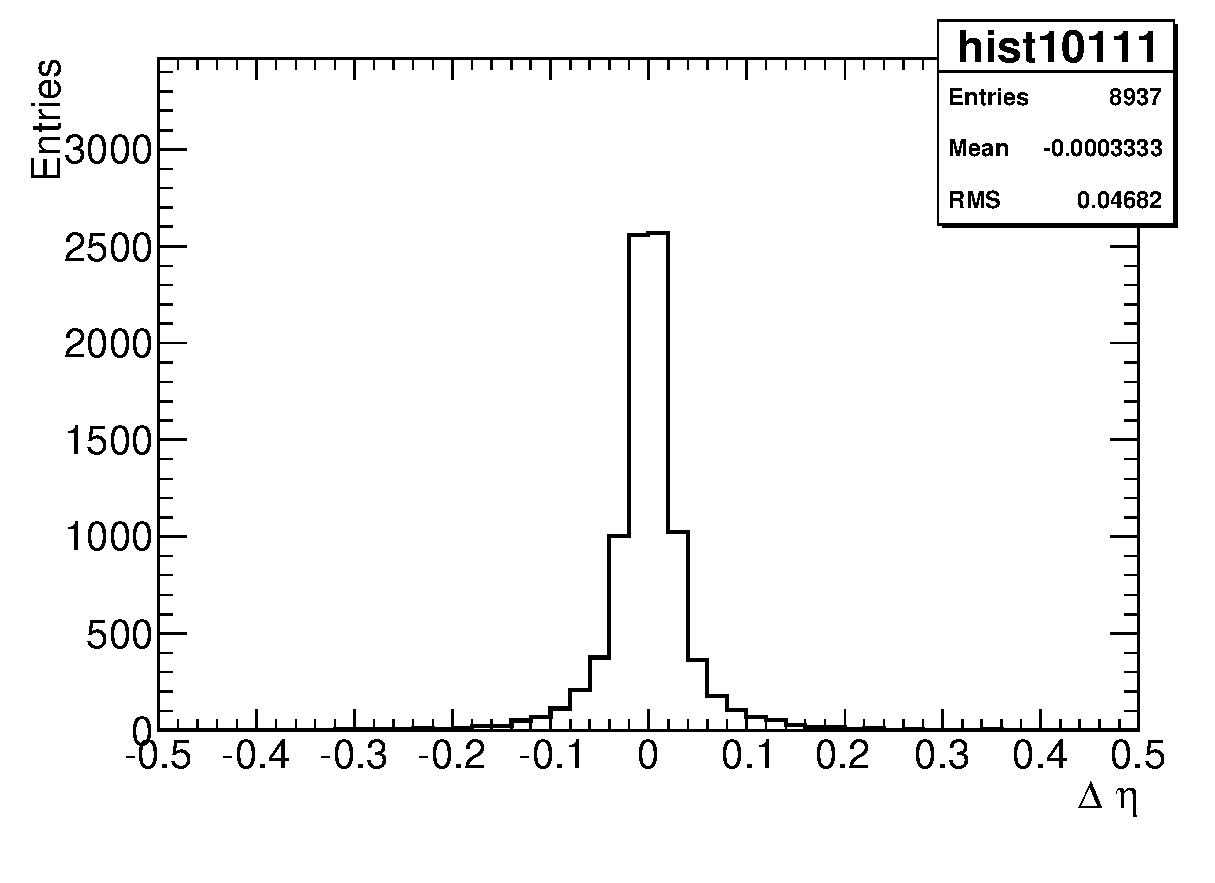
\includegraphics[width=7.0cm,angle=0]{plot-etaclu.eps}
   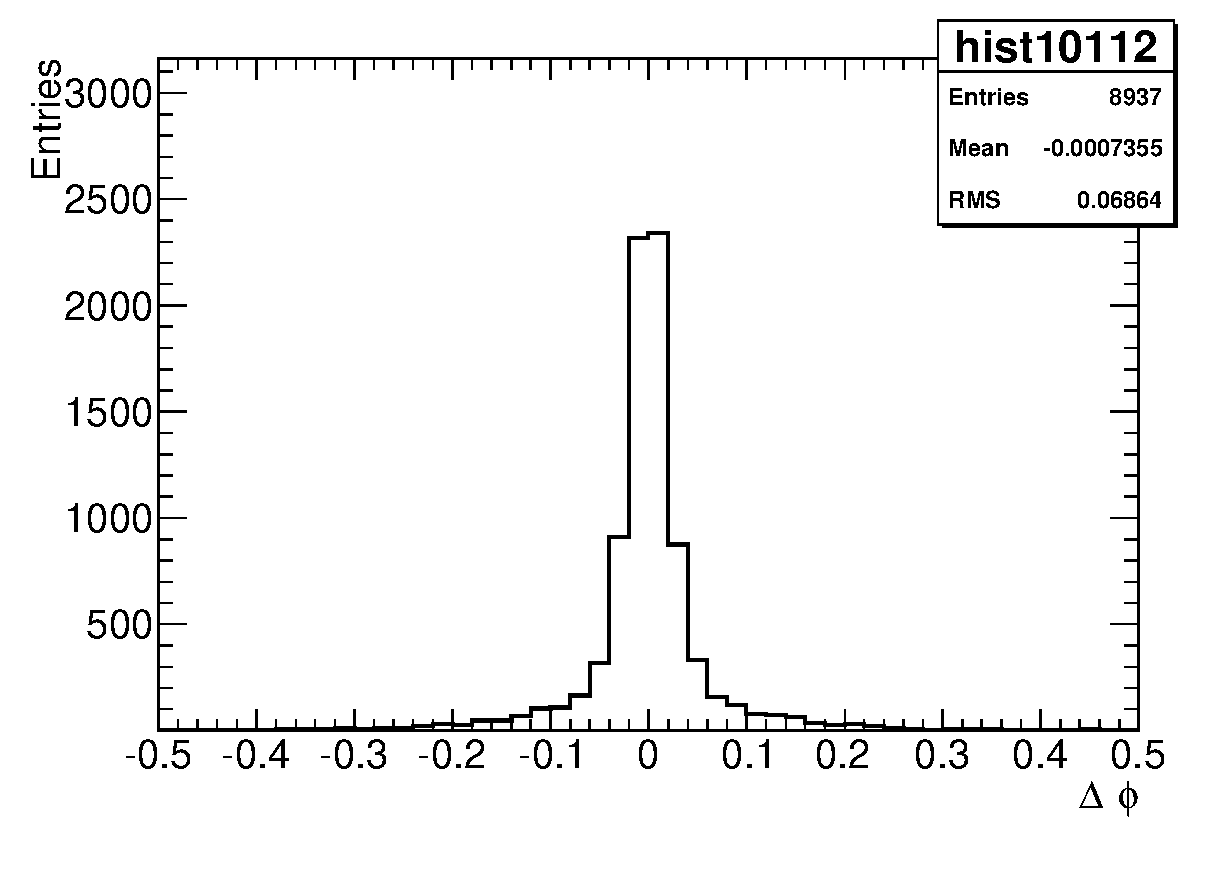
\includegraphics[width=7.0cm,angle=0]{plot-phiclu.eps}
\end{center}
\caption{\em
The $\Delta \eta$ (left) and  $\Delta \phi$ (right) distribution
between the reconstructed bary-center of particles falling within the
cluster cone  and the reconstructed cluster position. Shown are results 
for generated  $gg \to H, H \to u \bar u$ process with $m_H~=~125$~GeV.
\label{FS2.1}} 
\end{Fighere}


\boldmath 
%%%%%%%%%%%%%%%%%%%%%%%%%%%%%%%%%%%%%%%%%%%%%%%%%%%%
\subsection{Isolated muons}
%%%%%%%%%%%%%%%%%%%%%%%%%%%%%%%%%%%%%%%%%%%%%%%%%%%%
\unboldmath

Algorithm reconstructing isolated muons uses information
of the generated muons, reconstructed calorimetric clusters and
the cells map.

Isolated muon candidates are searched for in the container
{\tt InputRecord.particles}. The inverse muon four-momentum is
smeared according to the Gaussian resolution parametrised with
function {\tt Smearing::forMuon} (default: $\sigma = 0.05\% \cdot p_{T}$).
 The muon direction remains unsmeared.

For all muons which pass selection criteria in $p_T$ and $\eta$
(default: $p_T >$ 6 GeV and $|\eta| < 2.5$ GeV), isolation criteria,
in terms of the distance from calorimetric  clusters and of
maximum transverse energy 
deposition in cells in a cone around the muon, are then applied
(defaults: separation by $\Delta R > 0.4$ from other clusters and
$\sum E_T < 10$ GeV in a cone  $\Delta R = 0.2$ around the muon).
All muons passing the isolation criteria are stored in the container
{\tt OutputRecord.Muons} and those not passing are stored in
 {\tt OutputRecord.NonisolatedMuons}. 
 
As a control physics process  the
 $gg \to H \to ZZ^* \to 4 \mu $ production with the 
Higgs boson mass of 125 GeV is used. The default
isolation selection has 97.8\% efficiency for muons passing kinematical selection  with 
$p_T^{\mu_1, \mu_2} > 20$~GeV and $p_T^{\mu_3, \mu_4} > 7$~GeV. 
As the predicted intrinsic width
of the Higgs boson of this mass is very small, the resolution is
completely dominated by the resolution assumed for the 
single muon reconstruction. Fig.~\ref{FS2.4} (left) shows the
reconstructed distribution of the 4-muon system.
The assumed single muon transverse momenta resolution
 of $\sigma = 0.05\% \cdot p_T$
leads to the $\sigma_m = 1.57$~GeV resolution for the invariant mass
of the four-muon system originating from the $ H \to ZZ^* \to 4 \mu $
decay. Please note that the photon bremsstrahlung
was omitted in the event generation.



\begin{Fighere}
\begin{center}
   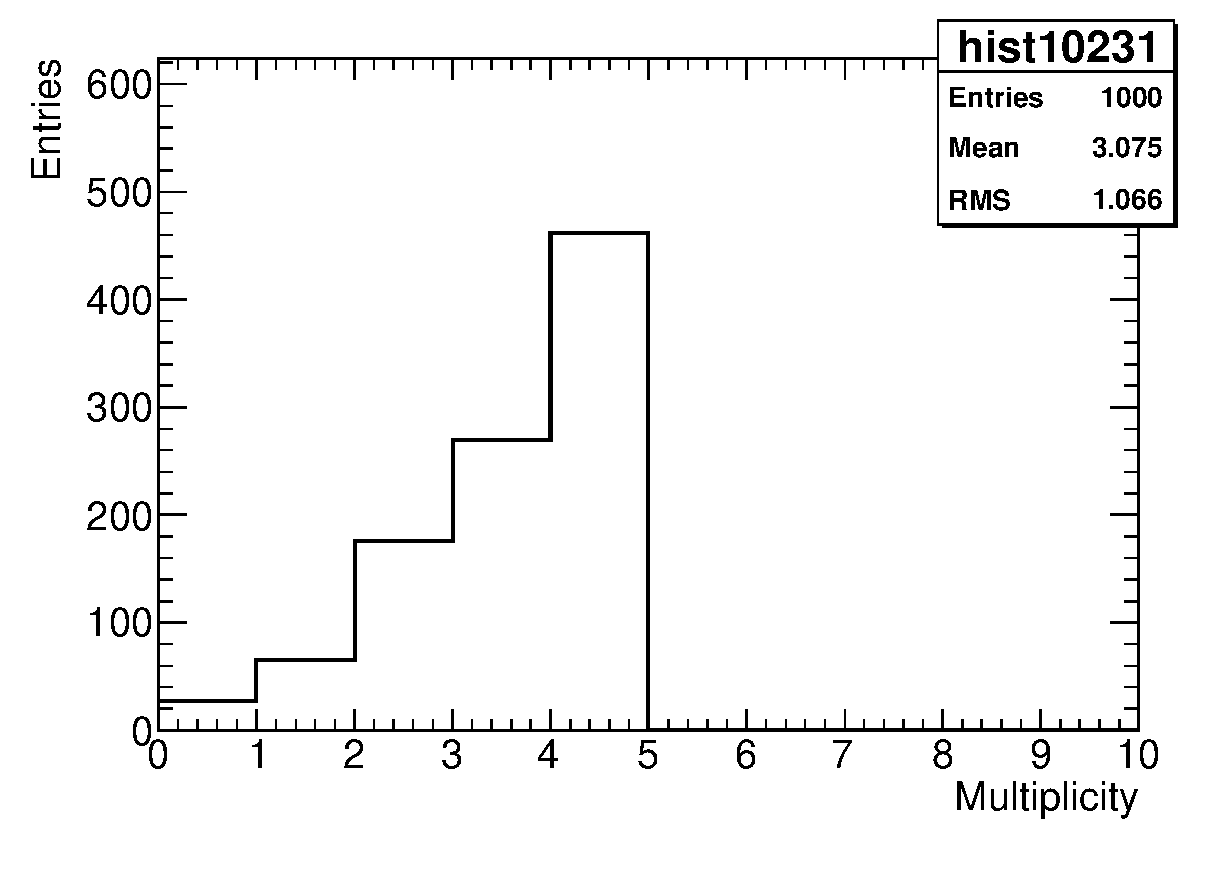
\includegraphics[width=7.0cm,angle=0]{plot-HPisolMuons.eps}
   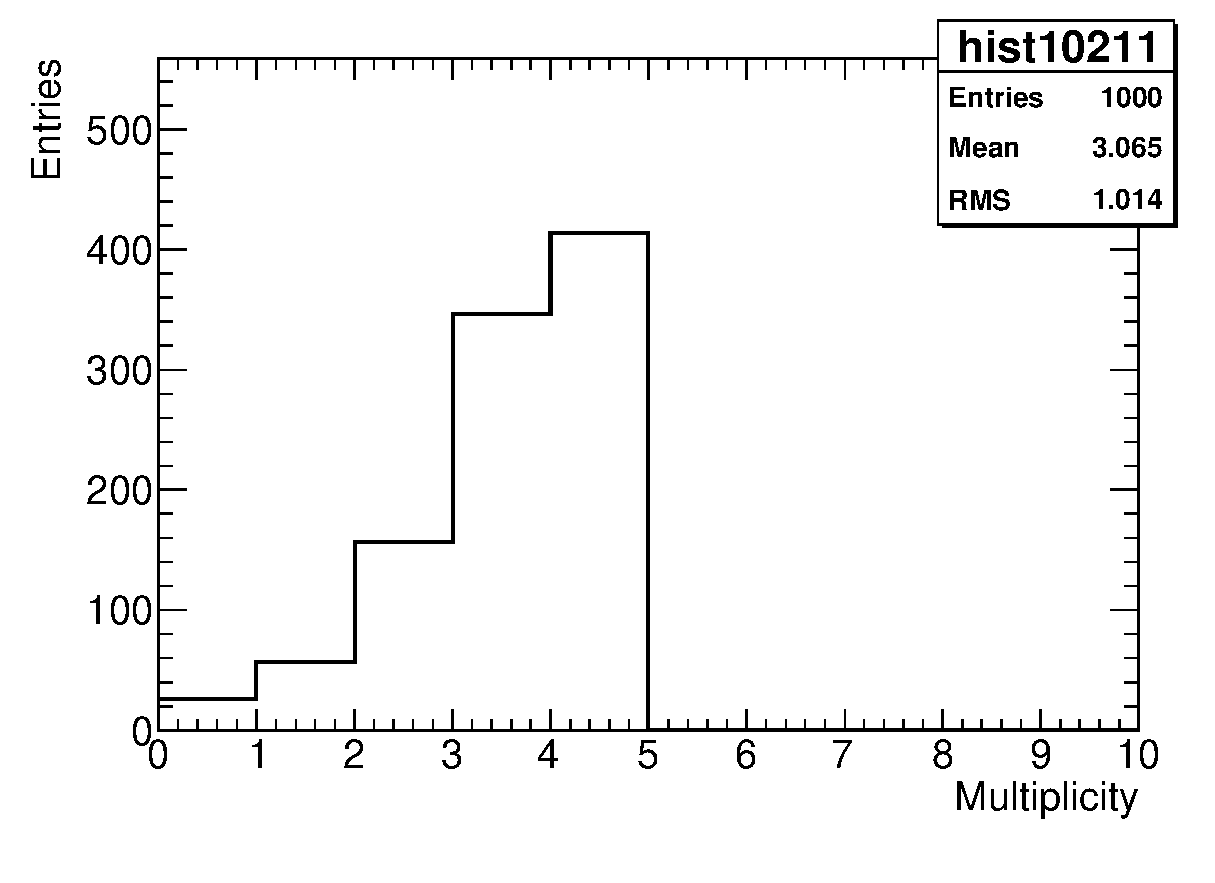
\includegraphics[width=7.0cm,angle=0]{plot-recoMuons.eps}
\end{center}
\caption{\em
Left: The multiplicity of  hard-process isolated muons (left) and reconstructed isolated muons (right) 
for $gg \to H, H \to ZZ^* \to 4\mu$ events with $m_H=125$~GeV.
\label{FS2.4}} 
\end{Fighere}


\boldmath 
%%%%%%%%%%%%%%%%%%%%%%%%%%%%%%%%%%%%%%%%%%%%%%%%%%%%
\subsection{Isolated electrons}
%%%%%%%%%%%%%%%%%%%%%%%%%%%%%%%%%%%%%%%%%%%%%%%%%%%%
\unboldmath

Algorithm reconstructing isolated electrons uses information
of the generated electrons, reconstructed calorimetric clusters and
the cells map.

Isolated electron candidates are searched for in the 
{\tt InputRecord.particles}. The electron four-momentum is
smeared according to the Gaussian resolution parametrised with
function {\tt Smearing::forElectron} (default: $\sigma = 12\%/\sqrt{E}$).
 The electron direction remains unsmeared.

For all electrons which pass selection criteria in $p_T$ and $\eta$
(default: $p_T >$ 5 GeV and $|\eta| < 2.5$ GeV), the associated 
reconstructed  calorimeter cluster is identified (default: $\Delta
R_{e, cluster} < 0.1$). Electron isolation criteria, in terms of
the distance from other clusters and of maximum transverse energy 
deposition in cells in a cone around the electron, are then applied
(defaults: separation by $\Delta R > 0.4$ from other clusters and
$\sum E_T < 10$ GeV in a cone  $\Delta R = 0.2$ around the electron).
All electrons passing the isolation criteria are stored in 
{\tt OutputRecord.Electrons} and the clusters associated with them are
removed from the {\tt  OutputRecord.Clusters}. 

As a control physics process  the
 $gg \to H \to ZZ^* \to 4e $ production with the 
Higgs boson mass of 125 GeV is used. The default
isolation selection has 95.2\% efficiency for electrons passing
kinematical selection  with 
$p_T^{e_1, e_2} > 20$~GeV and $p_T^{e_3, e_4} > 7$~GeV.
As the predicted intrinsic width
of the Higgs boson of this mass is very small, the resolution is
completely dominated by the resolution assumed for the 
single electron reconstruction. Fig.~\ref{FS2.3} (left) shows the
reconstructed distribution of the 4-electron system.
The assumed single electron energy resolution of $\sigma = 12\%/\sqrt{E}$
leads to the $\sigma_m = 1.26$~GeV resolution for the reconstructed invariant mass
of the four-electron system originating from the $ H \to ZZ^* \to 4e $
decay. Please note that the photon bremsstrahlung
was omitted in the events generation.



\begin{Fighere}
\begin{center}
   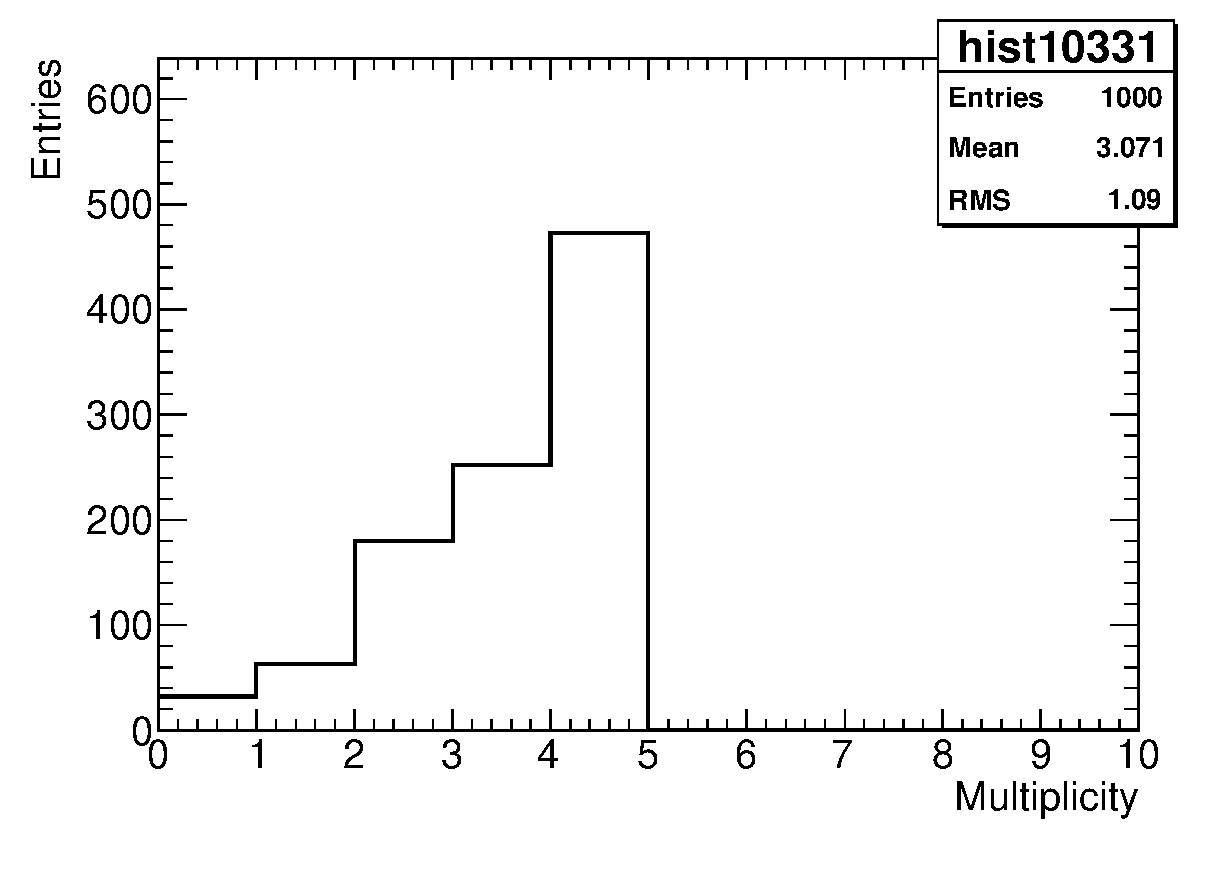
\includegraphics[width=7.0cm,angle=0]{plot-HPisolElectrons.eps}
   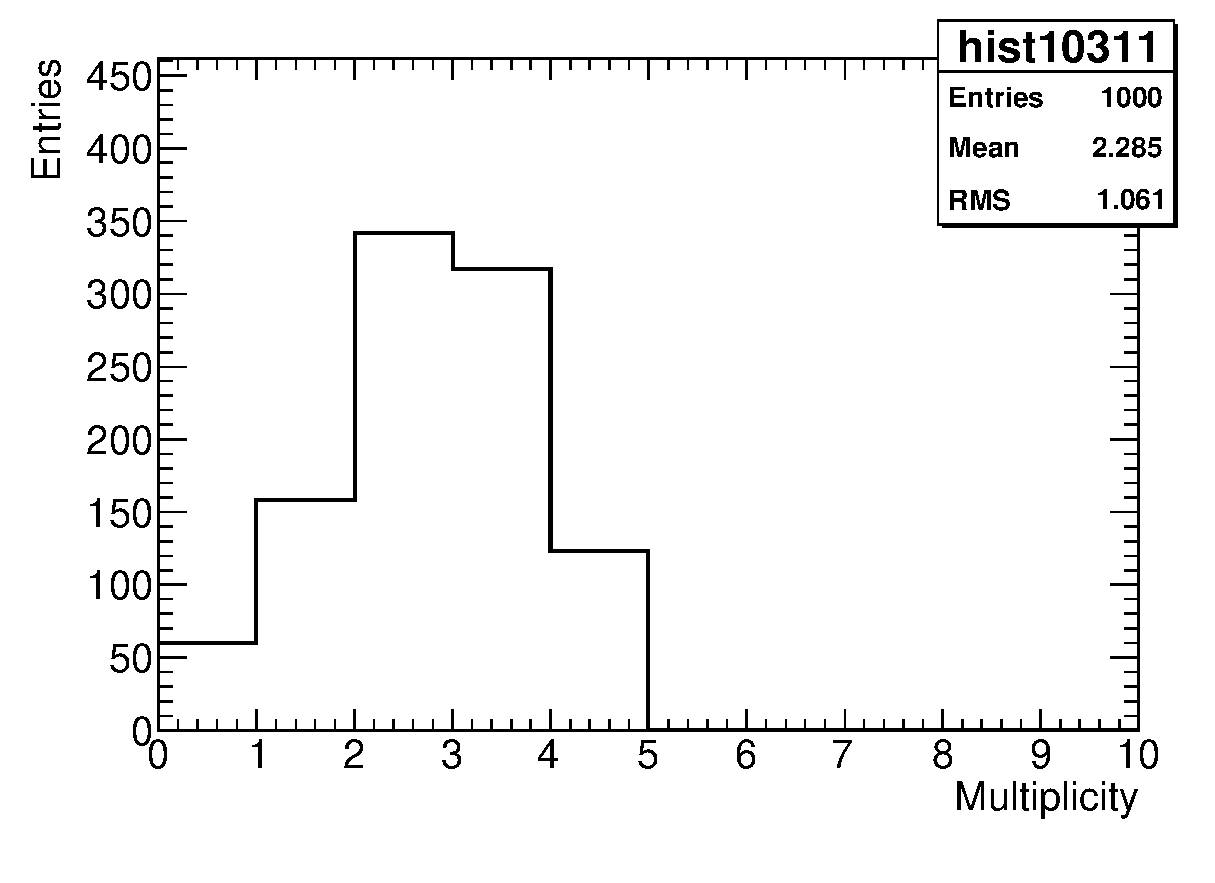
\includegraphics[width=7.0cm,angle=0]{plot-recoElectrons.eps}
\end{center}
\caption{\em
Left: The multiplicity of  hard-process isolated electrons (left) and reconstructed isolated electrons (right) 
for $gg \to H, H \to ZZ^* \to 4 e$ events with $m_H=125$~GeV.
\label{FS2.3}} 
\end{Fighere}


\boldmath 
%%%%%%%%%%%%%%%%%%%%%%%%%%%%%%%%%%%%%%%%%%%%%%%%%%%%
\subsection{Isolated photons}
%%%%%%%%%%%%%%%%%%%%%%%%%%%%%%%%%%%%%%%%%%%%%%%%%%%%
\unboldmath

Algorithm reconstructing isolated photons uses information
of the generated photons, reconstructed calorimetric clusters and
the cells map.
 
Isolated photon candidates are searched for in the 
{\tt  InputRecord.particles}. The photon four-momentum is
smeared according to the Gaussian resolution parametrised with
function {\tt Smearing::forPhoton} (default: $\sigma = 10\%/\sqrt{E}$).
The photon direction remains unsmeared.

For all photons which pass selection criteria in $p_T$ and $\eta$
(default: $p_T >$ 5 GeV and $|\eta| < 2.5$ GeV), the associated 
reconstructed  calorimeter cluster is identified (default: $\Delta
R_{\gamma, cluster} < 0.1$). Photon isolation criteria, in terms of
the distance from other clusters and of maximum transverse energy 
deposition in cells in a cone around the photon, are then applied
(defaults: separation by $\Delta R > 0.4$ from other clusters and
$\sum E_T < 10$ GeV in a cone  $\Delta R = 0.2$ around the photon).
All photons passing the isolation criteria are stored in 
{\tt OutputRecord.Photons} and the clusters associated with them are
removed from the {\tt OutputRecord.Clusters}. 

As a control physics process  the  Standard Model
$gg \to H \to \gamma \gamma$ production with the 
Higgs boson mass of 125 GeV is used. The 
isolation selection has 98.0\% efficiency for photons passing
the  kinematical selection of $p_T^{\gamma_1} > 40$ GeV and $p_T^{\gamma_2} > 25$ GeV.
As the predicted intrinsic width
of the Higgs boson of this mass is much below 1 GeV, the resolution 
of the reconstructed invariant mass of the di-photon system is
completely dominated by the resolution assumed for the 
single photon reconstruction. Fig.~\ref{FS2.2} (left) shows the
reconstructed distribution of the di-photon system of photons passing selection
criteria. The assumed energy resolution of $\sigma = 10\%/\sqrt{E}$
leads to the $\sigma_m = 0.85$ GeV resolution for the reconstructed
invariant mass of the di-photon system originating from the 
$ H \to \gamma \gamma$ decay.
 
\begin{Fighere}
\begin{center}
   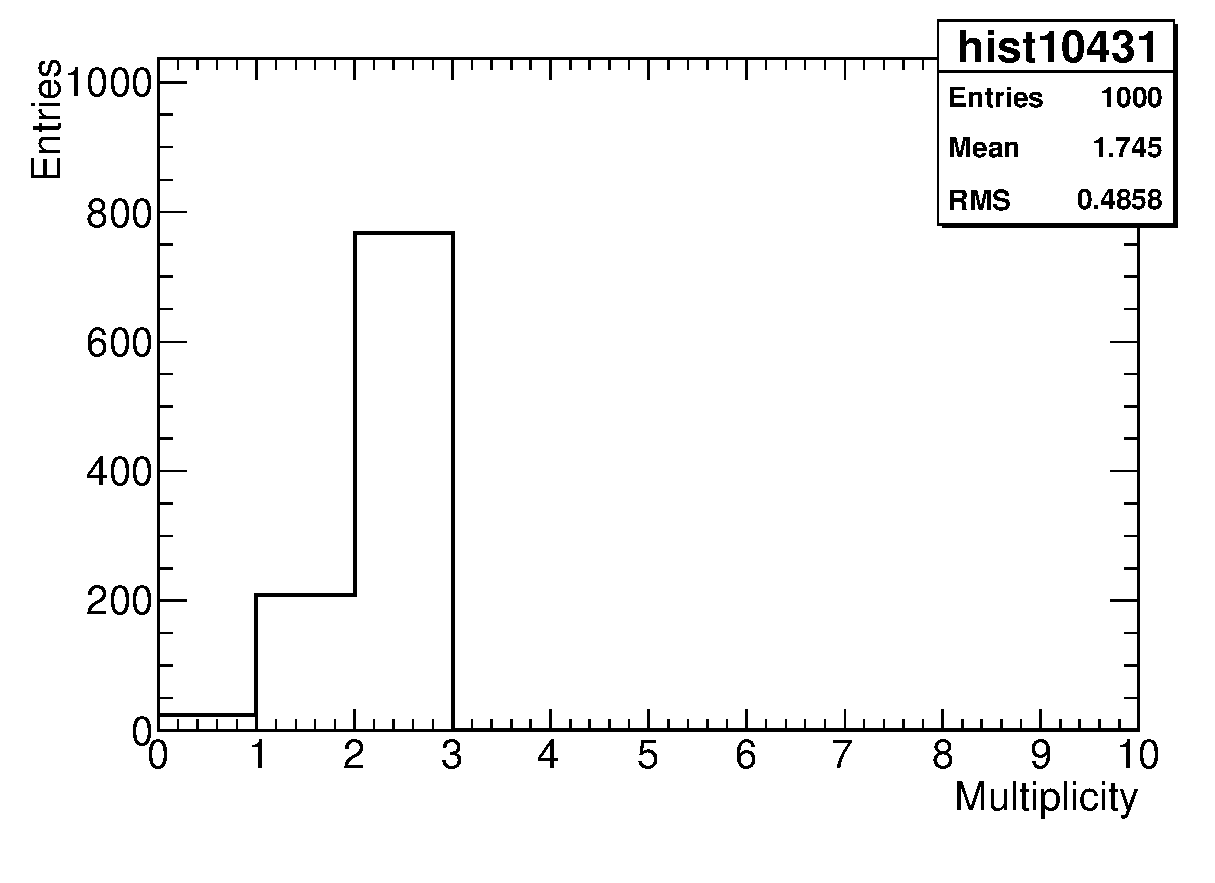
\includegraphics[width=7.0cm,angle=0]{plot-HPisolPhotons.eps}
   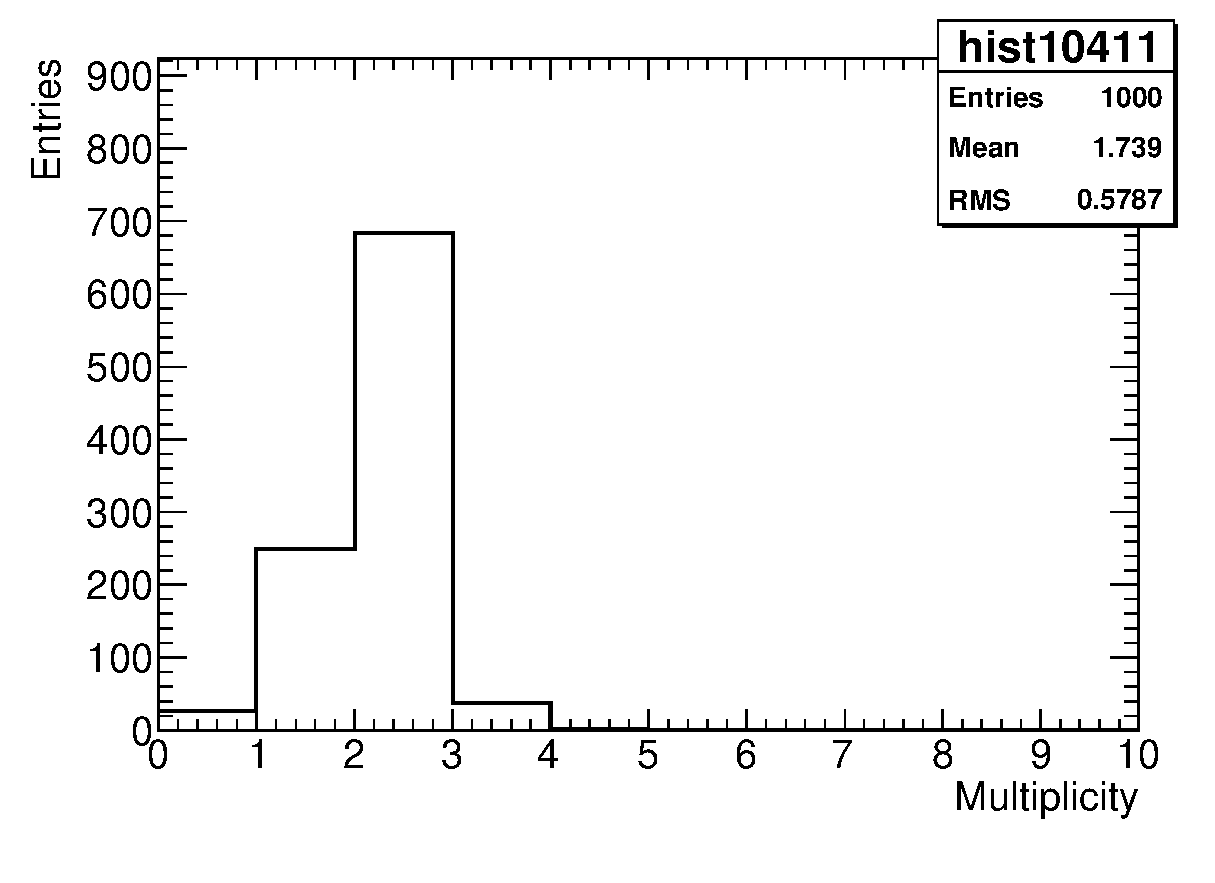
\includegraphics[width=7.0cm,angle=0]{plot-recoPhotons.eps}
\end{center}
\caption{\em
Left: The multiplicity of  hard-process isolated photons (left) and reconstructed isolated photons (right) 
for $gg \to H, H \to \gamma \gamma$ events with $m_H=125$~GeV.
\label{FS2.2}} 
\end{Fighere}


\boldmath 
%%%%%%%%%%%%%%%%%%%%%%%%%%%%%%%%%%%%%%%%%%%%%%%%%%%%
\subsection{Jets}
%%%%%%%%%%%%%%%%%%%%%%%%%%%%%%%%%%%%%%%%%%%%%%%%%%%%
\unboldmath

Clusters which have not been selected as associated with electrons or
photons are smeared with Gaussian resolution parametrised in function
{\tt Smearing::forHadron} (default: $\sigma = 50\%/\sqrt{E}$ and $100\%/\sqrt{E}$).
 

\begin{Fighere}
\begin{center}
{
   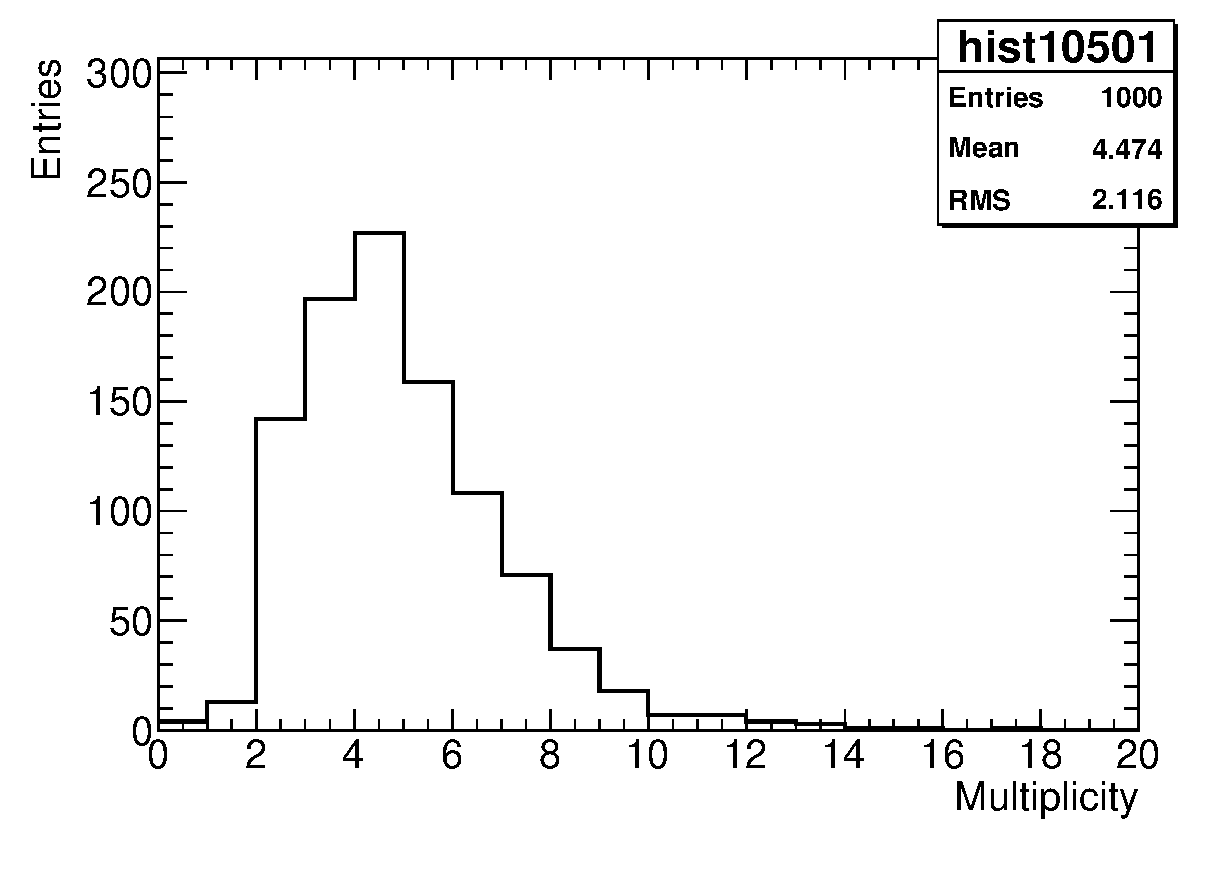
\includegraphics[width=7.0cm,angle=0]{plot-multiJets.eps}\\
}
{
   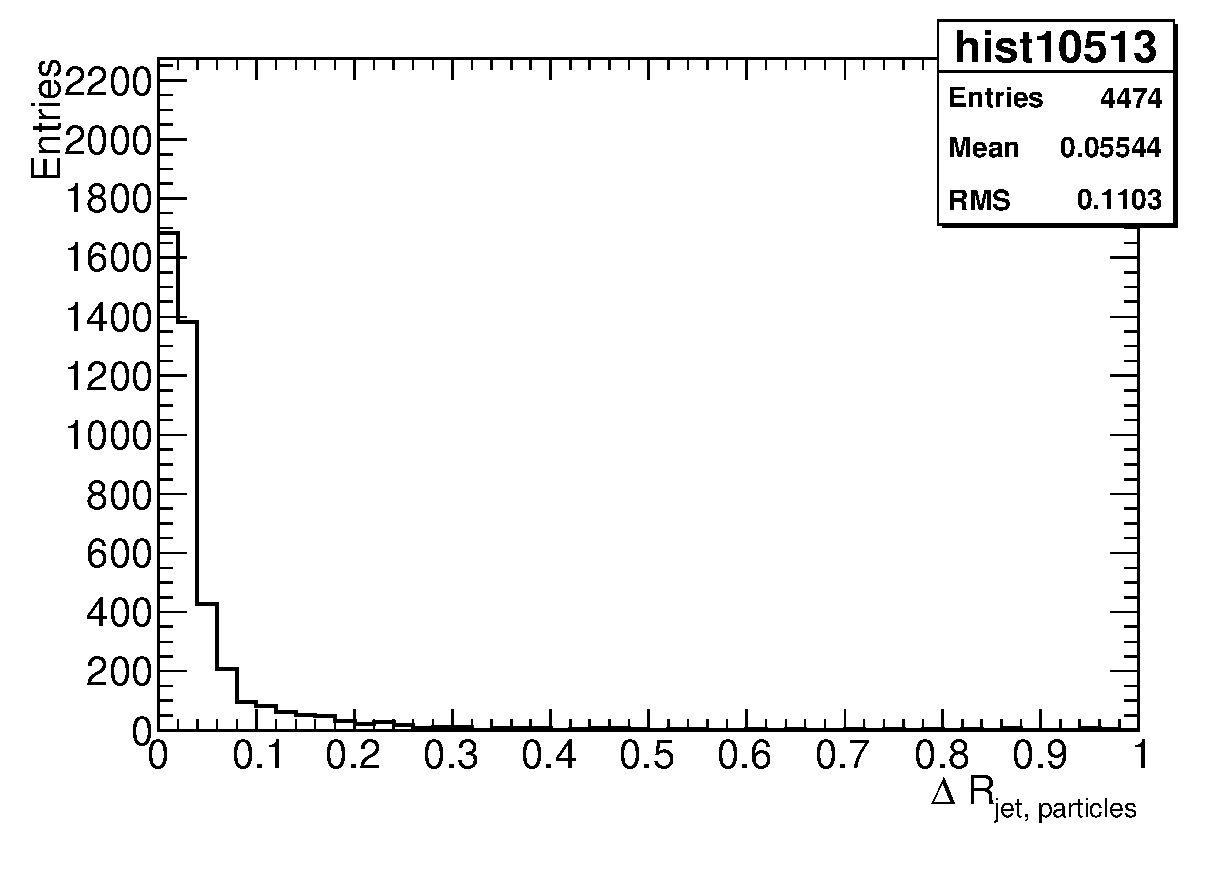
\includegraphics[width=7.0cm,angle=0]{plot-dR-jetParticles.eps}
   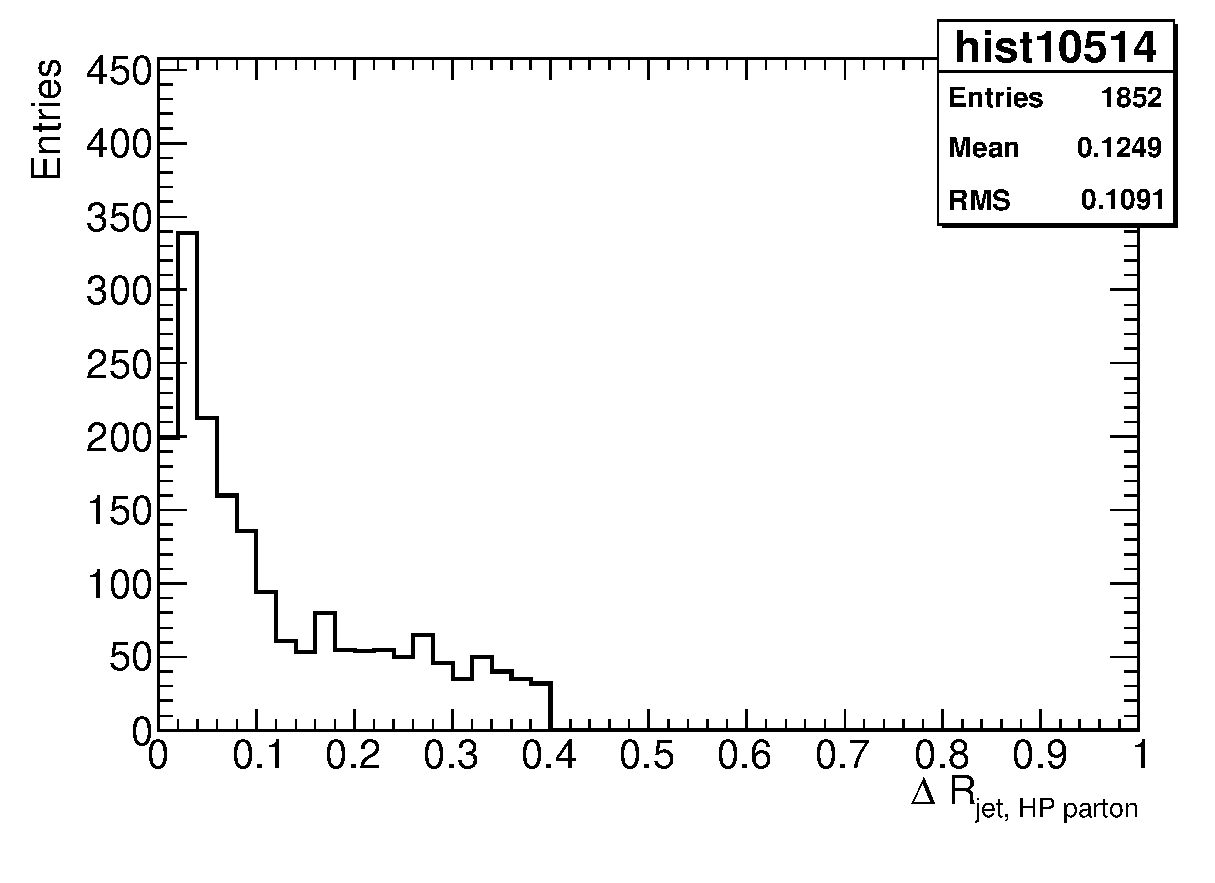
\includegraphics[width=7.0cm,angle=0]{plot-dR-jetHPparton.eps}\\
}
{
   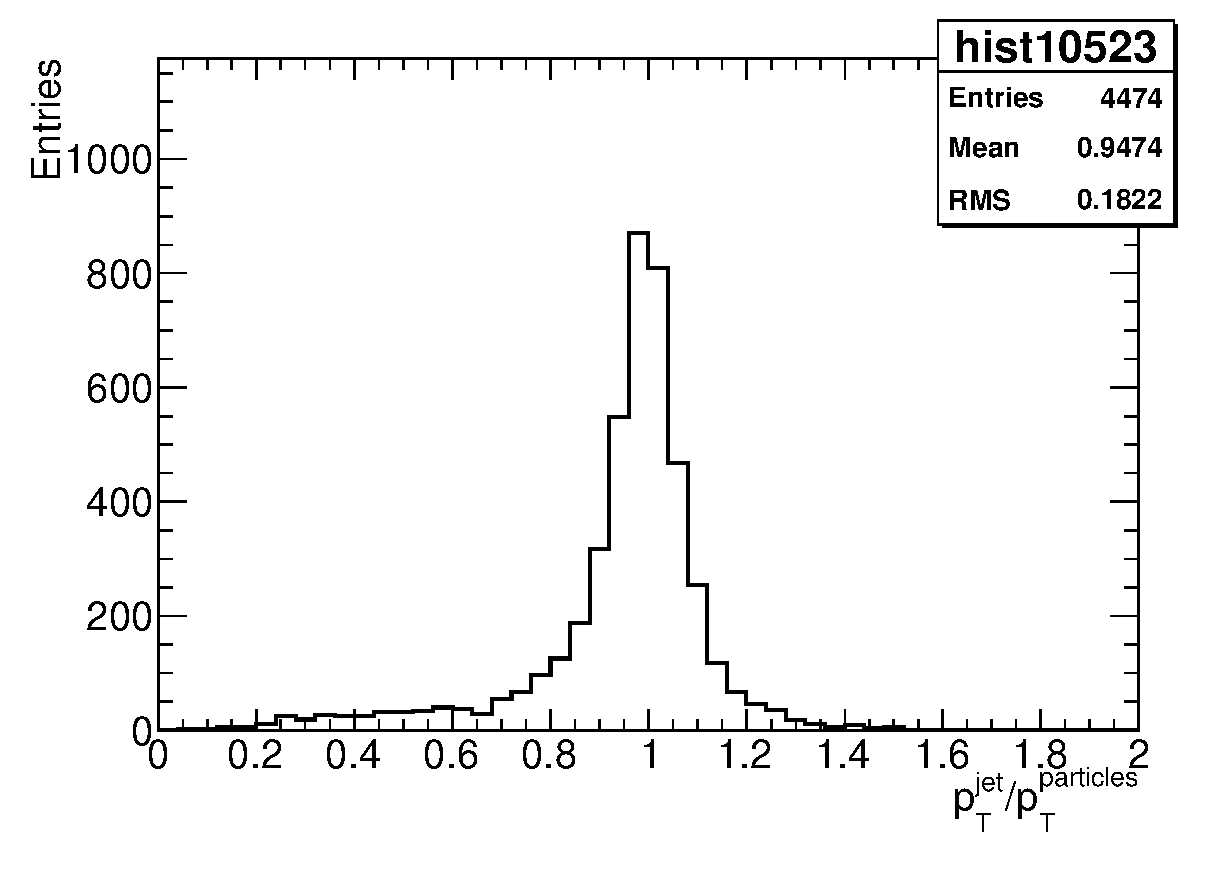
\includegraphics[width=7.0cm,angle=0]{plot-dPT-jetParticles.eps}
   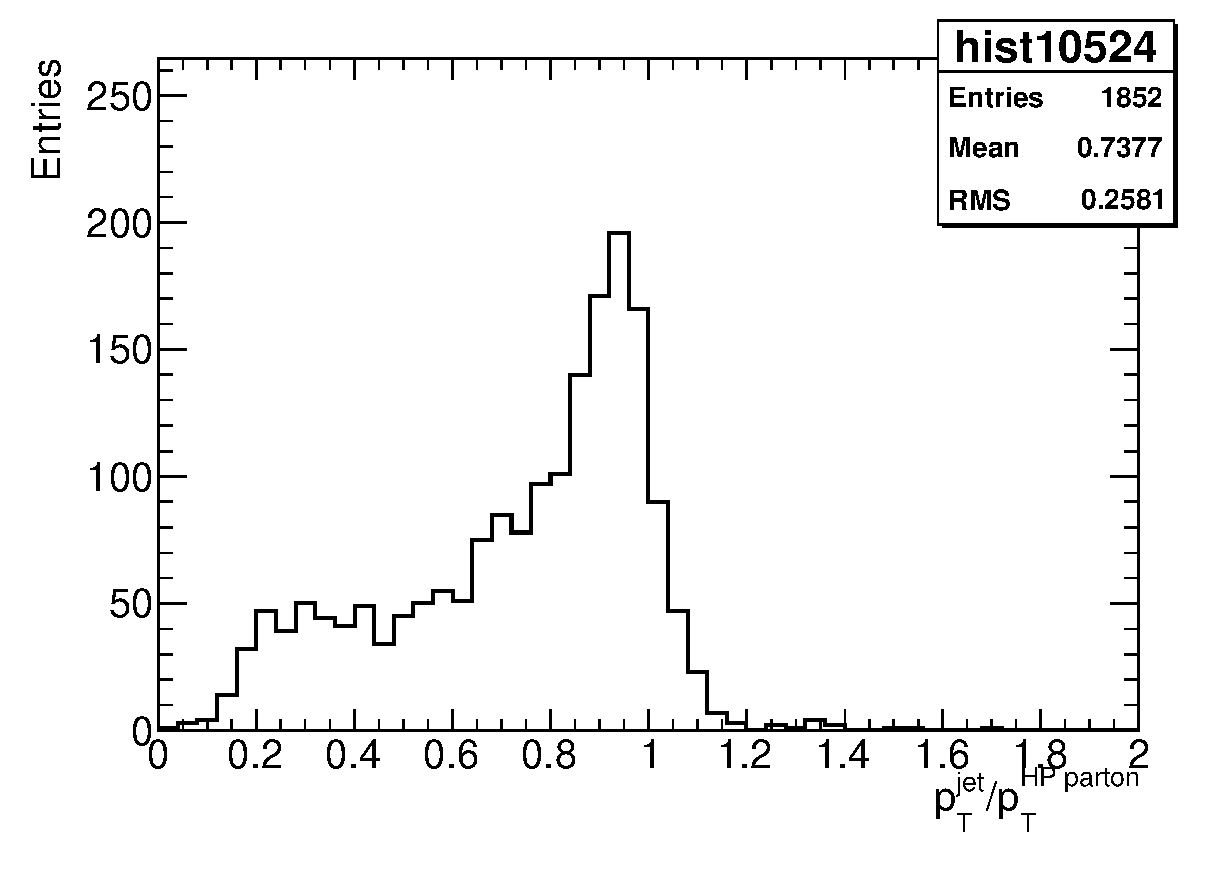
\includegraphics[width=7.0cm,angle=0]{plot-dPT-jetHPparton.eps}
}
\end{center}
\caption{\em
Multiplicity of jets (top), $\Delta R$ cone distance between reconstructed jet
and bary-center of particles (middle-left) and hard-process parton (middle right).
The ratio of $p_T^{jet}/p_T^{particles}$ (bottom-left) and
$p_T^{jet}/p_T^{HP parton}$ (bottom-right) for $gg \to H, H \to u \bar u$ and 
$m_{H} = 125$~GeV.
\label{FS2:5}} 
\end{Fighere}
\newpage


 If the non-isolated muon falls into the cone of a
cluster its 4-momenta  is added to the cluster 4-momenta and the
cluster direction is recalculated.
The resulting clusters are classified as jets if their transverse momentum
is greater than a given threshold (default: $p_T > 15$~GeV).
They are removed from the  {\tt OutputRecord.Clusters} and stored in the 
common  {\tt OutputRecord.Jets}.

The jets reconstruction efficiencies and di-jet mass resolution
have been studied using control physics process of the $WH$ production
with $m_H=125$~GeV and forcing the Higgs boson decay into specific
partons, namely $H \to u \bar u$, $H \to c \bar c$  and $H \to b \bar b$.
We used also process $gg \to H \to \tau \tau$ for estimating tau-jet
reconstruction efficiency (we forced tau-leptons decay into hadrons).
For estimating reconstruction efficiency we consider only jets which
have been reconstructed within the cone $\Delta R = 0.4$ from the
primary parton (particle) and we require that the primary parton
(particle) has passed
the same kinematical selection as required for reconstructed jets.

\boldmath 
%%%%%%%%%%%%%%%%%%%%%%%%%%%%%%%%%%%%%%%%%%%%%%%%%%%%
\subsubsection{Labeling}
%%%%%%%%%%%%%%%%%%%%%%%%%%%%%%%%%%%%%%%%%%%%%%%%%%%%
\unboldmath

Very important for the physics at LHC  are jets originating from b-quarks (so called
b-jets) which can be identified in the detector using b-tagging technique (vertex or
soft-lepton tags). The package labels a jet  as a b-jet if it is 
reconstructed within a limited rapidity
range (default: $|\Delta \eta| < 2.5$) and if a b-quark
of a transverse momenta (after FSR) above the threshold
(default: $p_T > 5$ GeV) is found within the cone 
(default: $\Delta R = 0.2$) around the axis of reconstructed jet.
The similar criteria are used for labeling the c-jets.

Equivalently important are also jets originating from the hadronic 
$\tau$-decay (so called $\tau$-jets) which can be identified using
dedicated algorithms.
The package labels jet as a tau-jet if the hadronic decay product is relatively
hard (default: $p_T^{\tau-had} > 10$ GeV), inside limited rapidity
range (default: $|\eta|<2.5$), dominates reconstructed jet transverse
momenta (default:  $p_T^{\tau-had}/p_T^{jet} > 0.9$), and is within
the cone (default: $\Delta R_{jet, \tau-had} < 0.3$) around the axis of a jet.  

Table~\ref{T2.1} summarises the jets reconstruction+labeling efficiencies as
obtained for the $WH, H \to b \bar b, c \bar c, u \bar u$ and
$gg \to H \to \tau \tau$ events.
Jets labeling is optional, can be switched off for b- and c-jets and/or separately
for tau-jets (default: ON).


\begin{Tabhere} 
\newcommand{\lstrut}{{$\strut\atop\strut$}}
  \caption {\em Efficiency for jet reconstruction+labeling for different types
  of initial partons with $p_T^{parton}> 15$ GeV (required 
  $p_T^{jet}> 15$ GeV). The rapidity coverage is limited to $|\eta| <2.5$.
  The $\Delta R_{cone}=0.4$ is used for cluster
  reconstruction and  $\Delta R_{cone}=0.2$ is used for matching
  criteria. The $WH, H \to b \bar b, c \bar c, u \bar u$ and $gg \to H
  \to \tau \tau$ processes were generated with $m_H = 125$ GeV.
In case of tau-jets only hadronic tau decays were generated.  
\label{T2.1}} 
\vspace{2mm}  
\begin{center}
\begin{tabular}{|c||c|} \hline \hline
Parton type & Reconstruction + Labeling  \\
\hline \hline
u-quark  &    95\%      \\
\hline
b-quark  &    81\%      \\
\hline
c-quark  &    87\%      \\
\hline
tau-jet  &    80\%      \\
\hline \hline
\end{tabular}
\end{center}
\end{Tabhere}


\begin{Fighere}
\begin{center}
{
   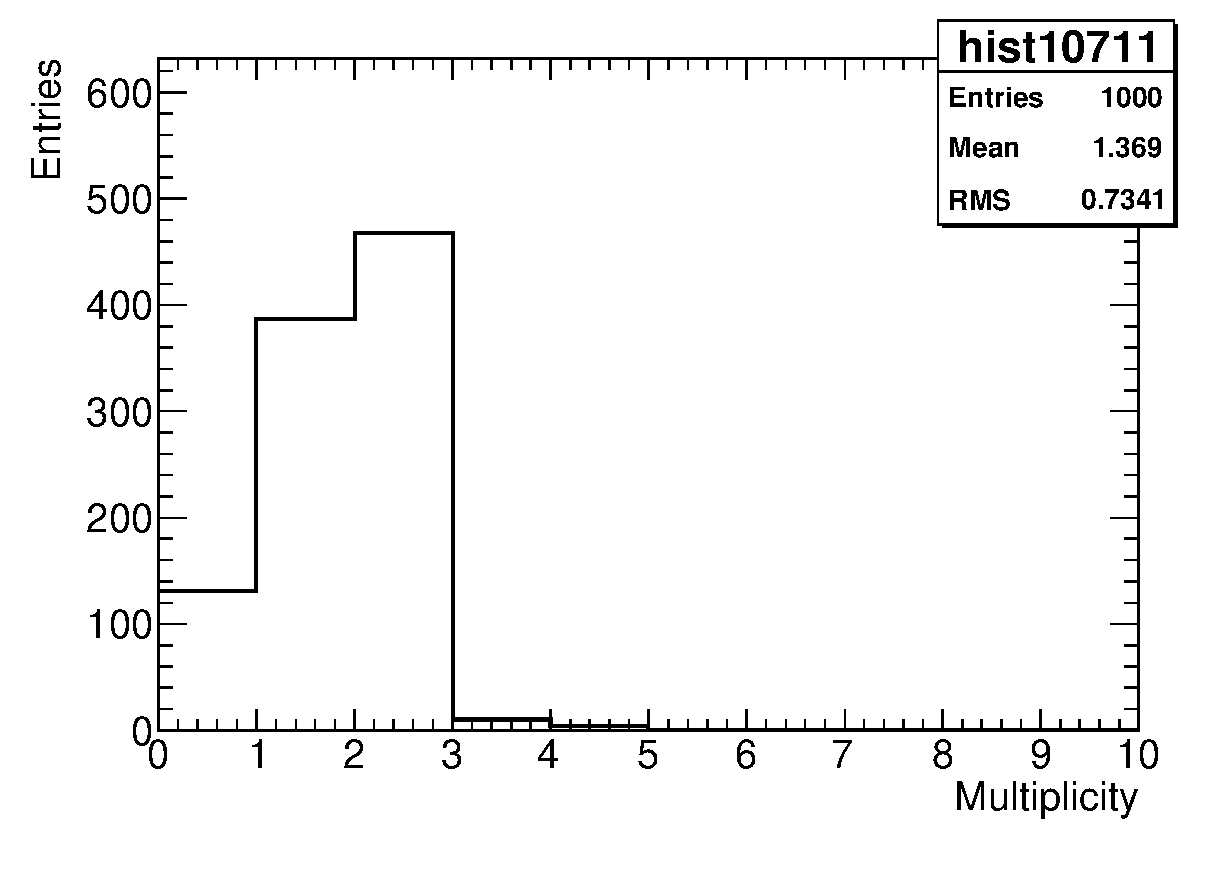
\includegraphics[width=7.0cm,angle=0]{plot-multiBJets.eps}
   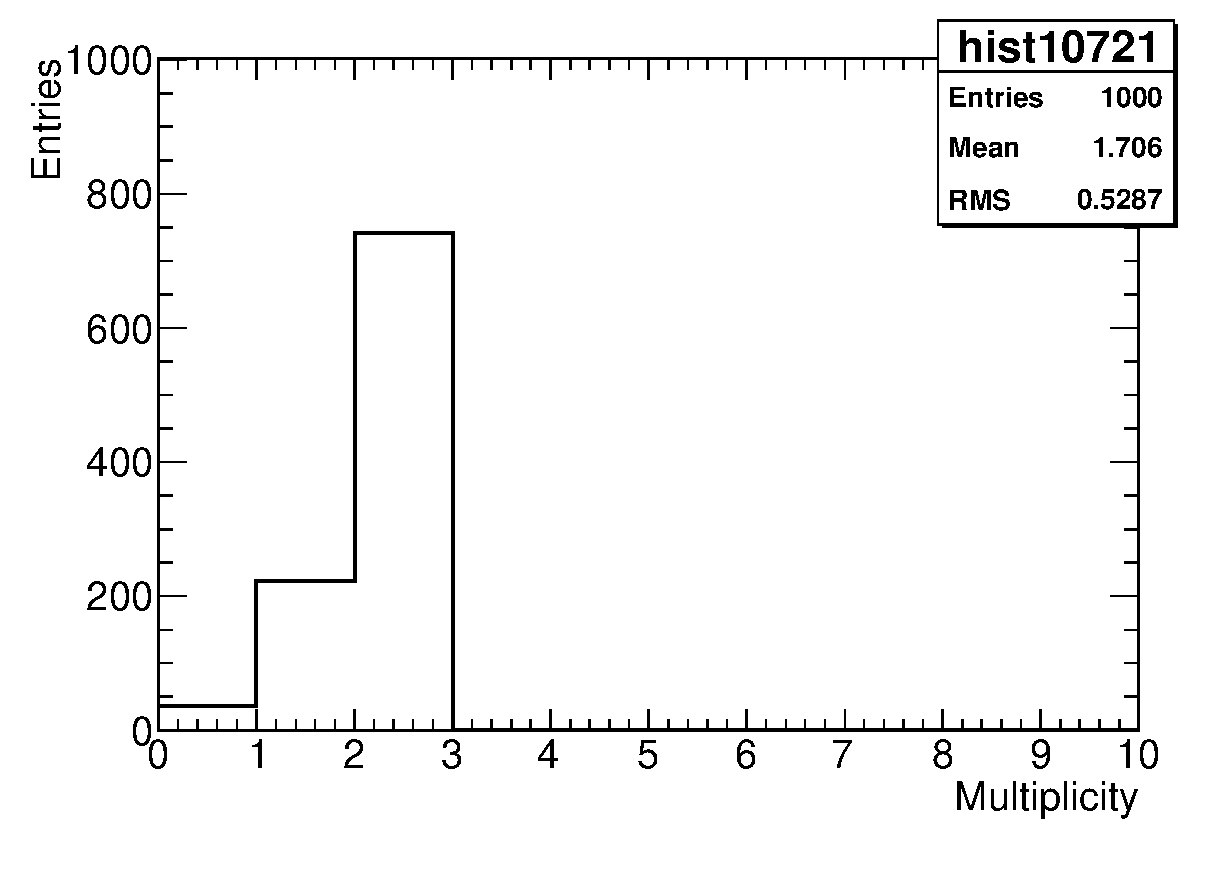
\includegraphics[width=7.0cm,angle=0]{plot-multiBquark.eps}\\
}
{
   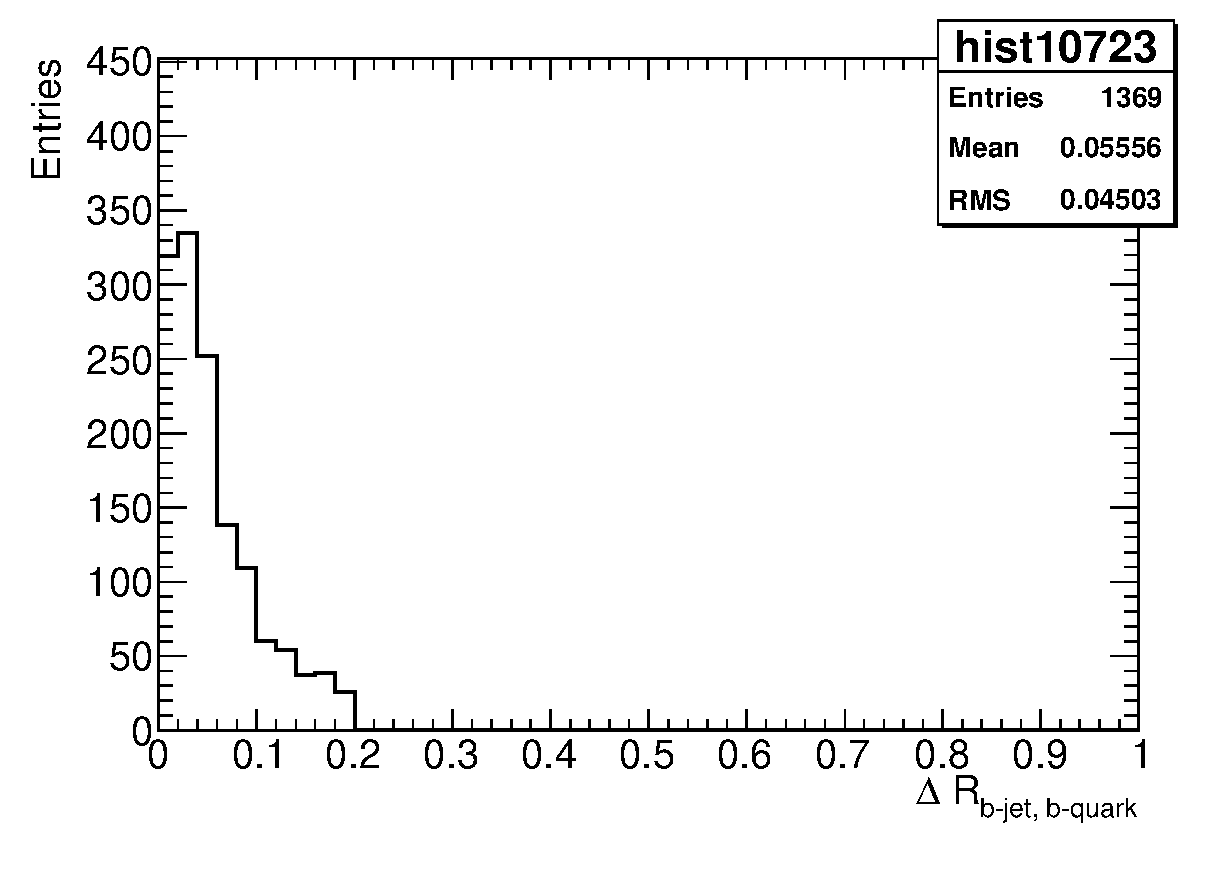
\includegraphics[width=7.0cm,angle=0]{plot-dR-bjetHPparton.eps}
   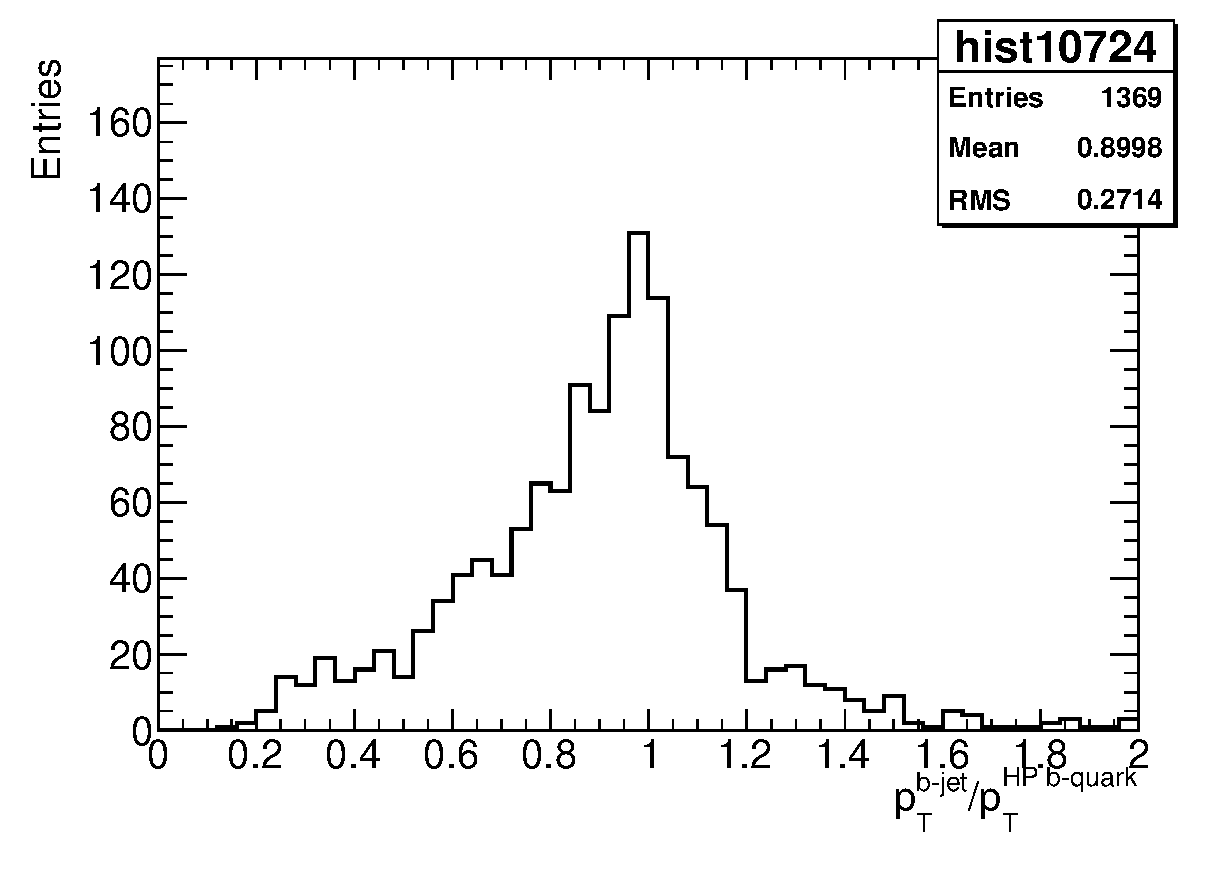
\includegraphics[width=7.0cm,angle=0]{plot-dPT-bjetHPparton.eps}
}
\end{center}
\caption{\em
Multiplicity of b-jets (top left) and hard-process b-quarks (top-right),
$\Delta R$ cone distance between b-labeled jet and hard-process b-quark (bottom-left);
the ratio of $p_T^{jet}/p_T^{HP b-quarks}$ (bottom-right). Distributions are shown
for $gg \to H, H \to b \bar b$ and  $m_{H} = 125$~GeV.
\label{FS2:5}} 
\end{Fighere}


\newpage
\begin{Fighere}
\begin{center}
{
   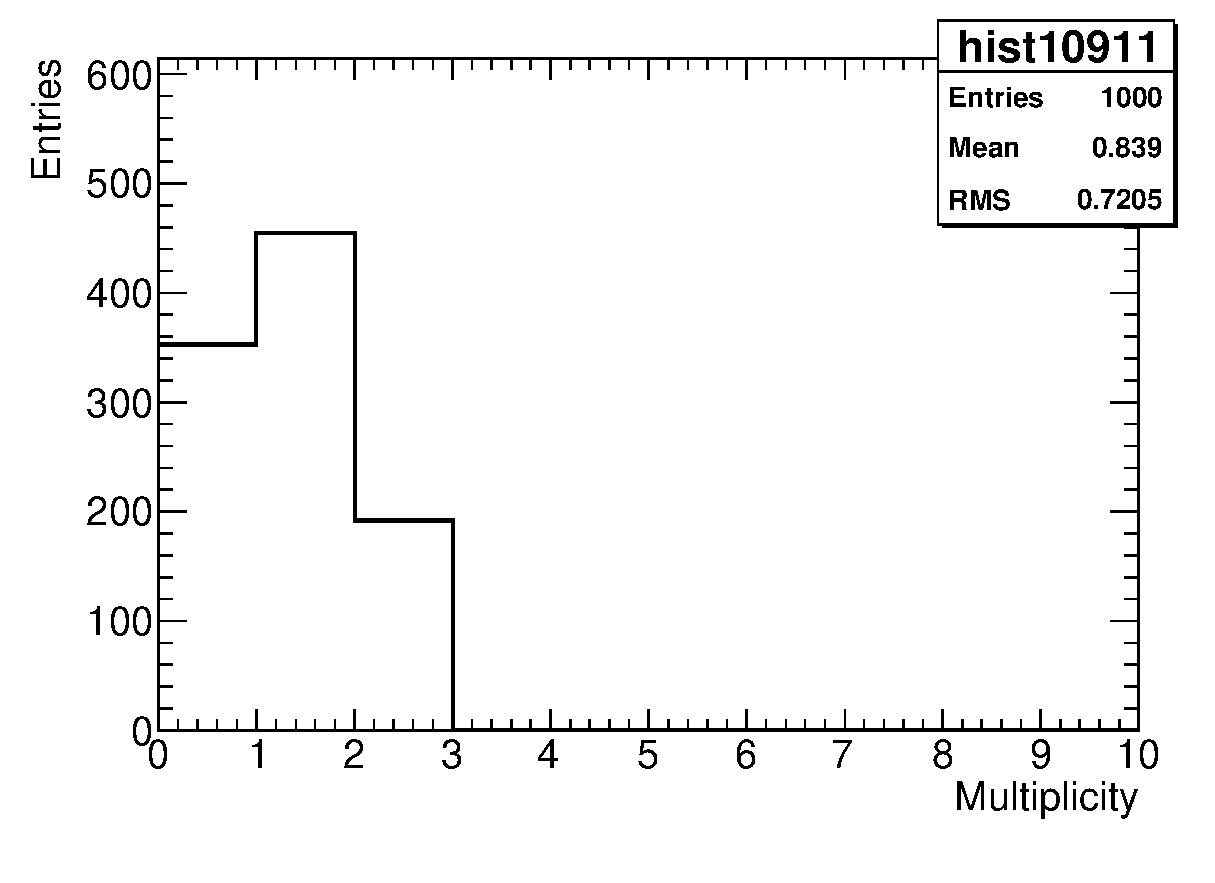
\includegraphics[width=7.0cm,angle=0]{plot-multiTauJets.eps}
   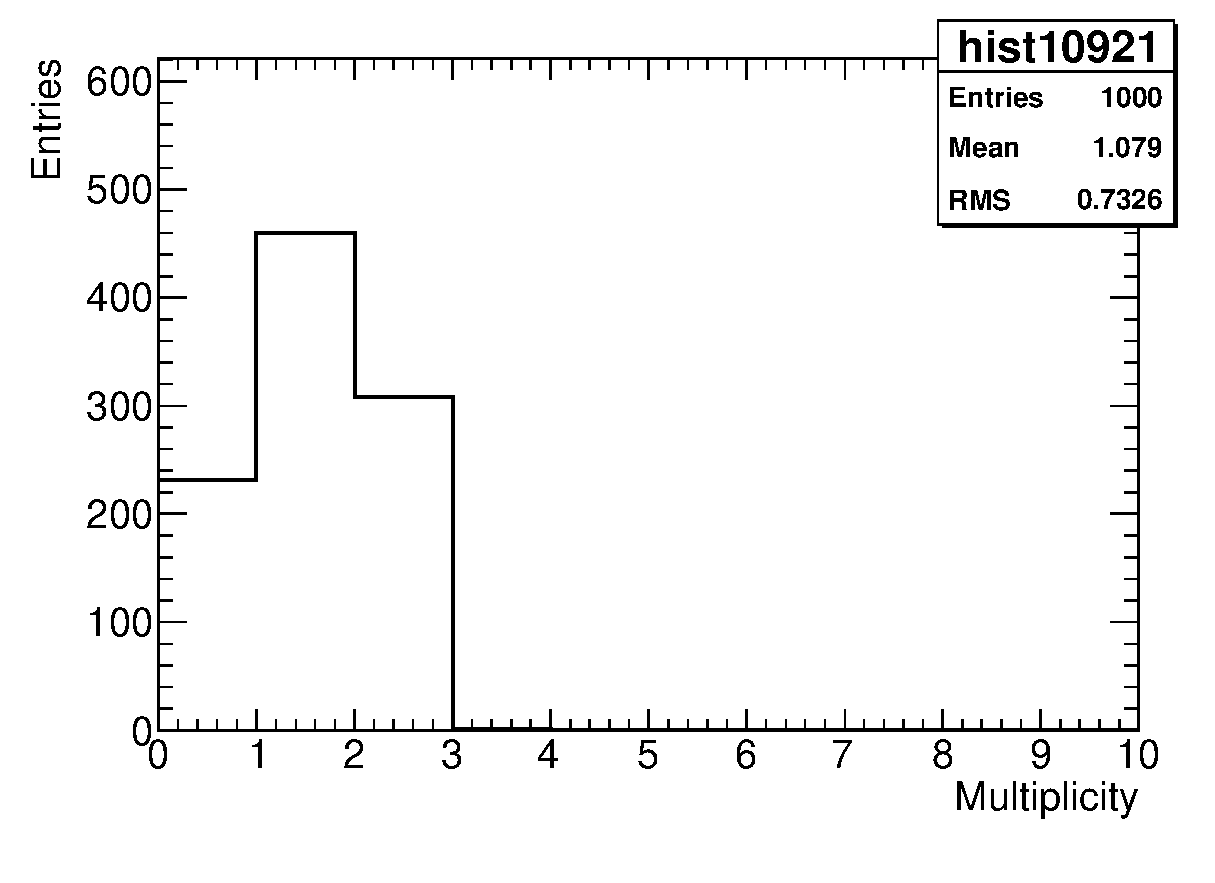
\includegraphics[width=7.0cm,angle=0]{plot-multiTauHP.eps}\\
}
{
   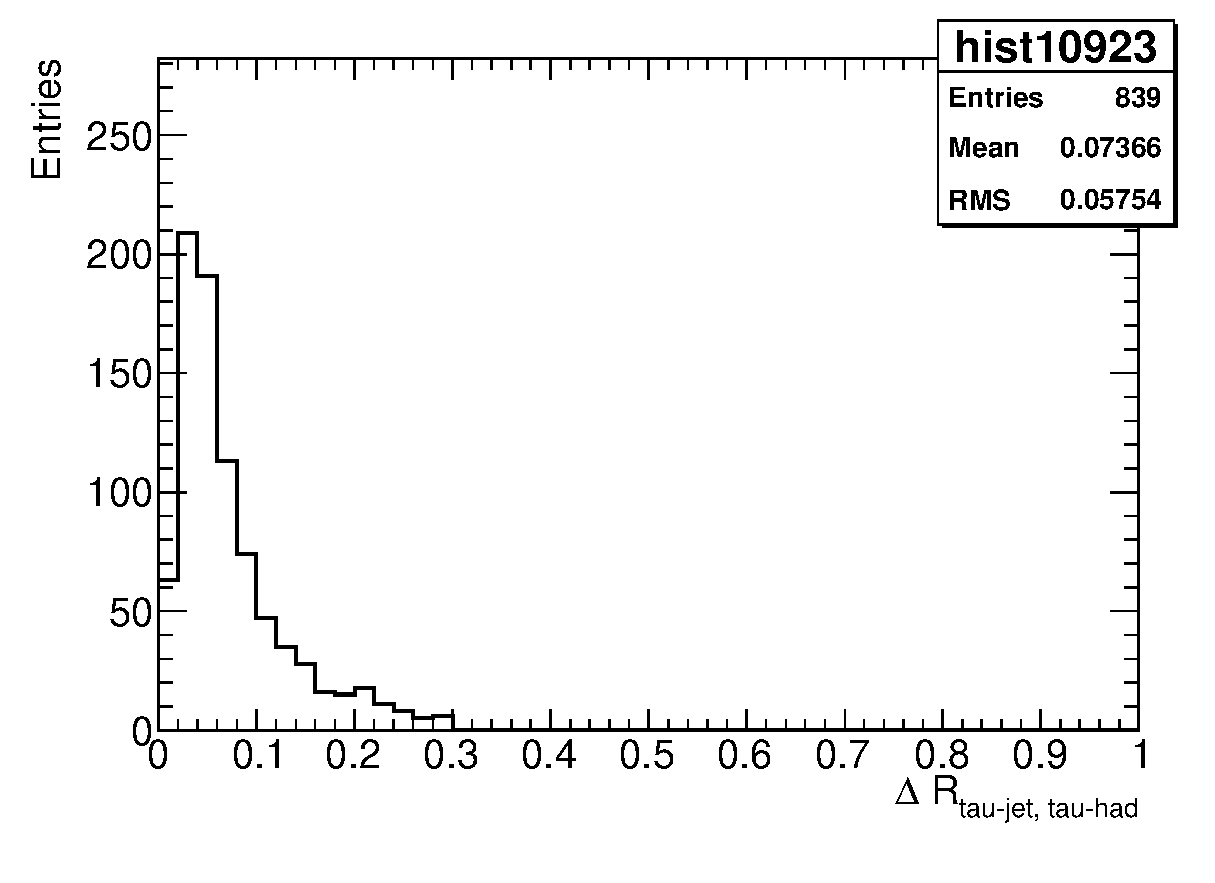
\includegraphics[width=7.0cm,angle=0]{plot-dR-jetTauHP.eps}
   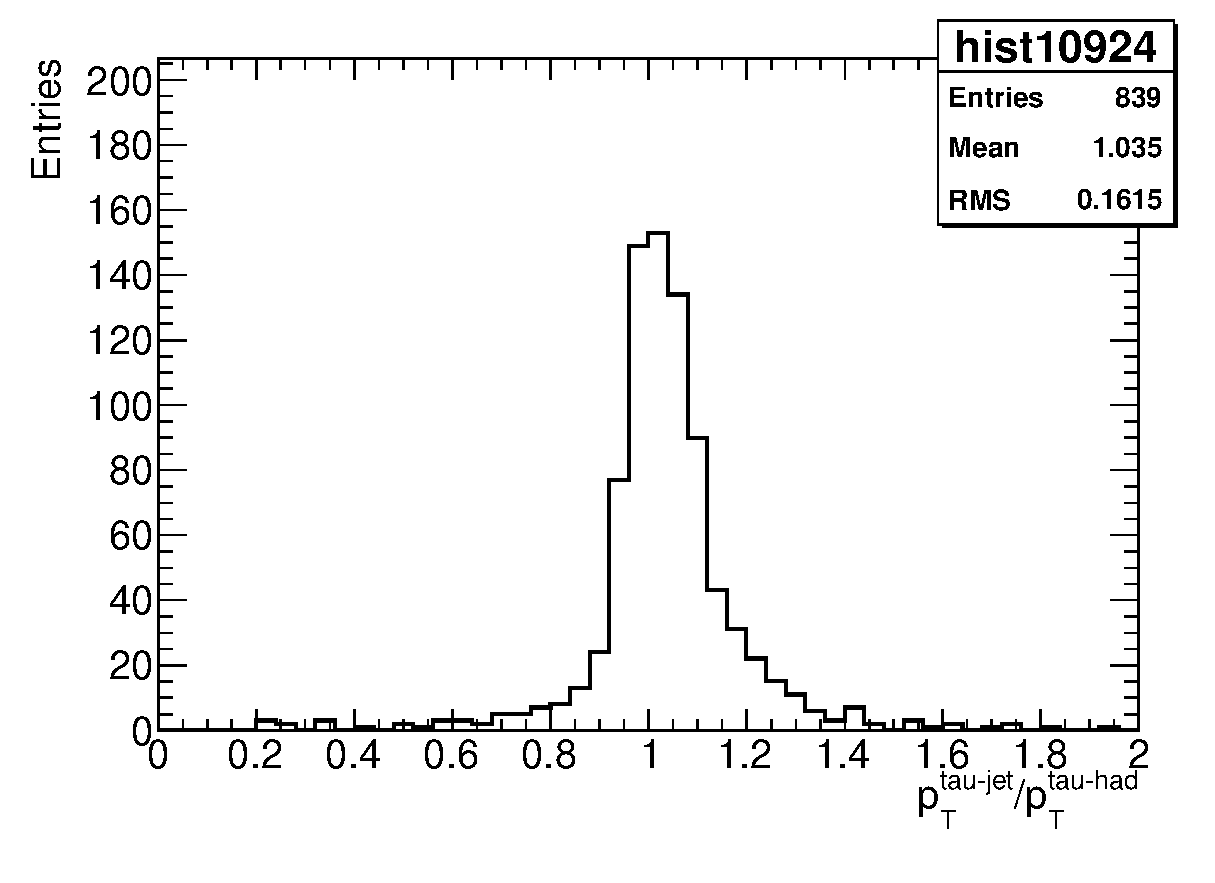
\includegraphics[width=7.0cm,angle=0]{plot-dPT-jetTauHP.eps}
}
\end{center}
\caption{\em
Multiplicity of tau-jets (top left) and hadronic tau (top-right),
$\Delta R$ cone distance between tau-labeled jet and hard-process tau-had (bottom-left);
the ratio of $p_T^{tau-jet}/p_T^{tau-had}$ (bottom-right). Distributions are shown
for $gg \to H, H \to \tau \tau$ and  $m_{H} = 125$~GeV.
\label{FS2:5}} 
\end{Fighere}

\boldmath 
%%%%%%%%%%%%%%%%%%%%%%%%%%%%%%%%%%%%%%%%%%%%%%%%%%%%
\subsubsection{Calibration}
%%%%%%%%%%%%%%%%%%%%%%%%%%%%%%%%%%%%%%%%%%%%%%%%%%%%
\unboldmath

The reconstructed jets four-momenta need to be 
 corrected for the out-cone energy
loss (cascade outside the jet-cone) and for the loss of the particles
escaping detection (those below threshold at $p_T=0.5$ GeV, neutrinos,
invisible particles, muons outside acceptance range or 
below the observability threshold).
Such correction, called calibration, can be performed on the
statistical basis only.
The single default calibration function (the same for any type of
jets), as a function of transverse momenta 
of reconstructed jet, $p_T^{jet}$,  is provided in the package.
The calibration algorithm corrects jets four-momenta
 without altering their direction.
Calibration can be switched off (default: ON). 

The quality of the calibration algorithm can be verified by monitoring
the ratio of $p_T^{b-quark}/p_T^{b-jet}$, taking into account
a hard-process quark which originates a given jet.
One can note, (see Fig.~\ref{FS2:5}, bottom plots) 
 that the implemented calibration function has a tendency to
undercalibrate b-jets while calibrates reasonably well u-jets. We can
observe also rather large tail in the $p_T^{jet}/p_T^{b-quark}$
distribution, caused by the semileptonic b-quarks decays and larger
spread of the cascading particles than in the  case of light jets.

As an effect of the hadronisation and cascading decays, the expected
resolution for the resonance reconstruction in the hadronic channels
will be much worse than in the leptonic ones.
The precision for reconstructing the peak position of the 
invariant mass  of the di-jet system will relay on the 
precision of the calibration procedure.


\boldmath 
%%%%%%%%%%%%%%%%%%%%%%%%%%%%%%%%%%%%%%%%%%%%%%%%%%%%
\subsection{Missing transverse energy}
%%%%%%%%%%%%%%%%%%%%%%%%%%%%%%%%%%%%%%%%%%%%%%%%%%%%
\unboldmath

The missing transverse energy is calculated by summing the transverse
momenta of identified isolated photons, electrons and muons, of jets
and clusters not accepted as jets and of
non-isolated muons not added to any jet. Finally, the
transverse energies deposited in cells not used for clusters
reconstruction are also included in the total sum. Transverse energies
deposited in unused cells are smeared with the same energy resolution
function as for jets, and cells with deposited transverse energy below
a given threshold (default: 0 GeV) are excluded from the sum. From
the calculation of the total sum $E_T^{obs}$ the missing transverse
energy is obtained, $E_T^{miss} =  E_T^{obs}$ as well as the missing
transverse momentum components $p_x^{miss} = - p_x^{obs}$, 
$p_y^{miss} = - p_y^{obs}$. The total calorimeter transverse energy,
$\sum E_T^{calo}$, is calculated as the sum of all the above
transverse energies except that of muons.
Please note, that missing transverse energy is calculated from the
energy balance before jets calibration is performed, as the possible 
out-cone energy loss is already taken into account by summing up energy
deposition of unused cells/clusters.

Fig.~\ref{FS2:7} shows the resolution of the transverse missing energy
obtained for the di-jet events generated with the transverse momenta
of the hard process above 17 GeV.

\begin{Fighere}
\begin{center}
{
   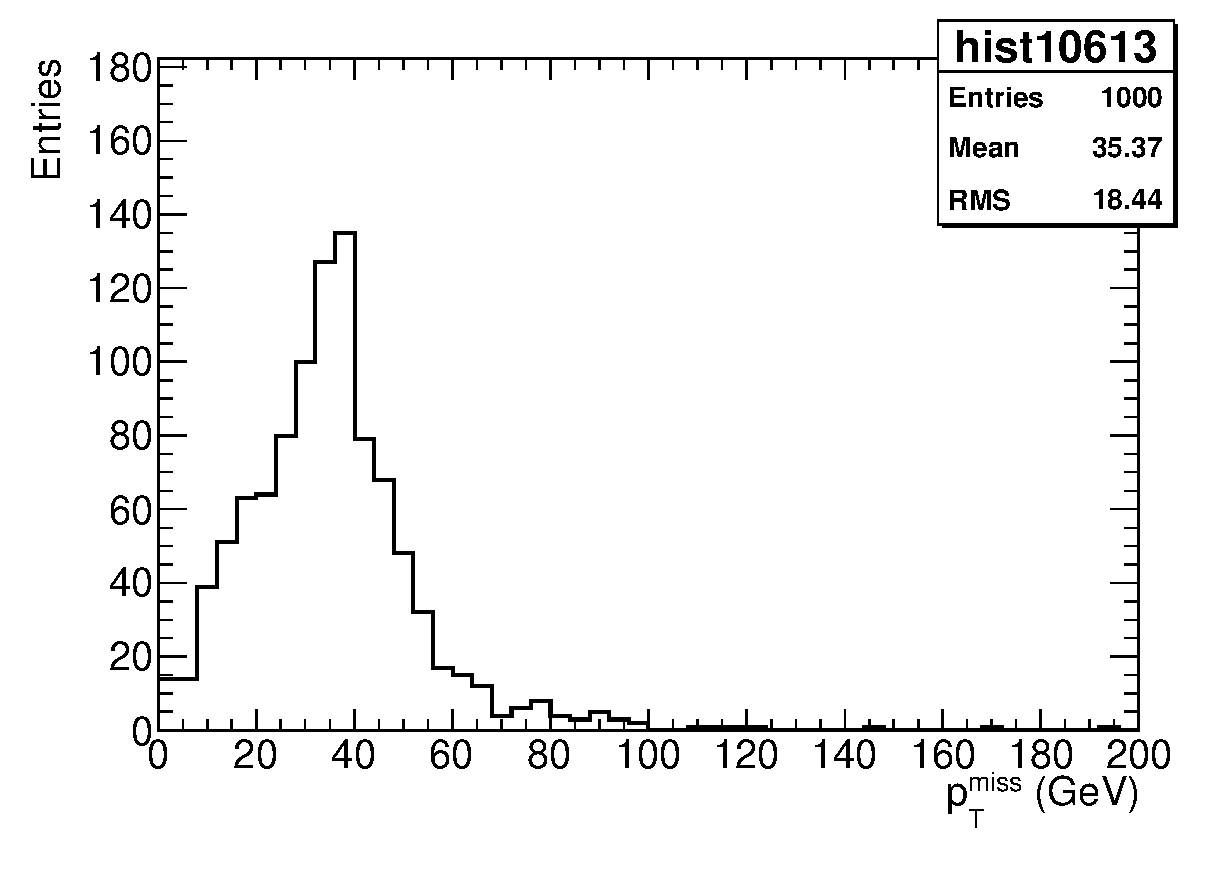
\includegraphics[width=7.0cm,angle=0]{plot-recoPTMiss.eps}
   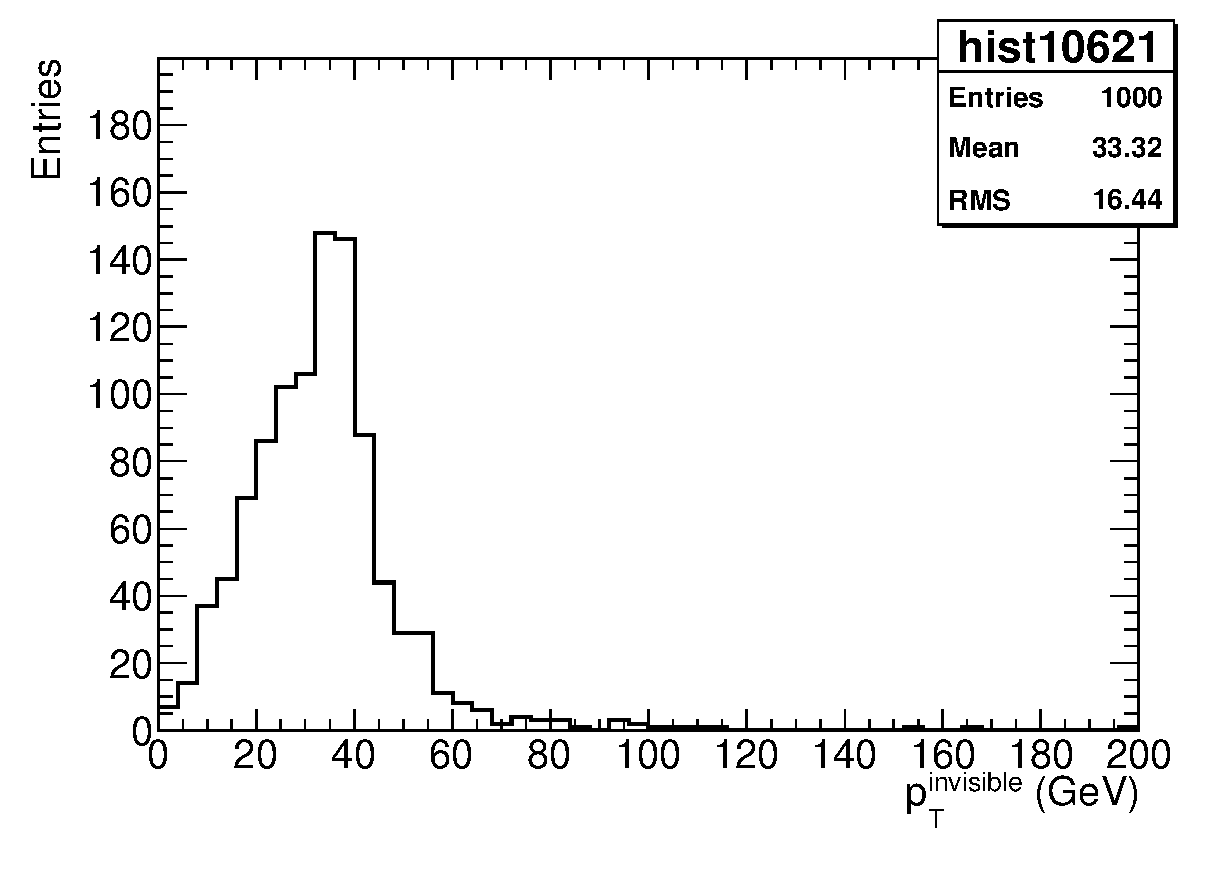
\includegraphics[width=7.0cm,angle=0]{plot-truthPTinvis.eps}\\
}
\end{center}
\caption{\em
The reconstructed missing transverse energy (left) and transverse momenta on neutrino
in $W \to e \nu$ events.
\label{FS2:7}} 
\end{Fighere}



\boldmath 
%%%%%%%%%%%%%%%%%%%%%%%%%%%%%%%%%%%%%%%%%%%%%%%%%%%%
\subsection{Additional efficiencies}
%%%%%%%%%%%%%%%%%%%%%%%%%%%%%%%%%%%%%%%%%%%%%%%%%%%%
\unboldmath

The algorithms of the {\tt AcerDET} package are not correcting for
inefficiencies of photon, electron and muon reconstruction and
identification. To be more realistic, one should apply a weighting
factor of 70\%-90\% for each isolated lepton used in the analysis and of
80\% for each isolated photon.

The package is also not correcting for tagging-efficiencies, namely
the labeling procedure is not equivalent to the b- and tau-jet
identification in the experiment. One can assume b-tagging efficiency 
of 60\% per b-labeled jet with mistagging probability of 10\% for
c-labeled jet and 1\% for the light jet.
For the tau-jets using efficiency of 50\% (per tau-labelled jet)
and 5 - 10 \% mistagging probability for other jets could be a reasonable
assumptions. One should be well aware that what proposed above 
represents quite crude estimates.

The package is also not correcting for trigger efficiencies which has
to be applied in addition if a given reconstructed object is foreseen to
trigger an event. 

\boldmath 
%%%%%%%%%%%%%%%%%%%%%%%%%%%%%%%%%%%%%%%%%%%%%%%%%%%%
\subsection{OUTPUT format}
%%%%%%%%%%%%%%%%%%%%%%%%%%%%%%%%%%%%%%%%%%%%%%%%%%%%
\unboldmath

By the end of the simulation and reconstruction algorithm,
reconstructed entities: photons, electrons, muons, jets, transverse
missing energy are available as collections of objects in the {\tt OutputRecord}.
Provided is algorithm to store this information in the {\tt ROOT} \cite{ROOT}
tree. However, the user might decide to
use his preferred data-base technology for storing output from the 
simulation and reconstruction algorithms.





\boldmath 
%%%%%%%%%%%%%%%%%%%%%%%%%%%%%%%%%%%%%%%%%%%%%%%%%%%%
\section{Outlook}
%%%%%%%%%%%%%%%%%%%%%%%%%%%%%%%%%%%%%%%%%%%%%%%%%%%%
\unboldmath

We presented package which can be useful for several
phenomenological studies on the high $p_T$ physics at LHC.
As example of more recent publications which have been using
its fortran version AcerDET-1.0 \cite{AcerDET-1.0} are papers eg. 
\cite{Nagata2015, Schaetzel2014, Choi2012, Aguilar-Saavedra2012},
for the more complete list see link \cite{AcerDET-1.0-citations}. 

It is not the aim of the package to represent in details performance of
neither ATLAS nor CMS detectors, nevertheless some global features
of these would be reproduced well. In particular we believe that the
analyses performed with the package for physics at LHC will be more
realistic than parton-level studies alone.

The package allows also for rather flexible 
adjusting of several key parameters which characterise features of any
detector for LHC or future ILC or FFC experiments. 


%%%%%%%%%%%%%%%%%%%%%%%%%%%%%%%%%%%%%%%%%%%%%%%%
\section*{Acknowledgments}
%%%%%%%%%%%%%%%%%%%%%%%%%%%%%%%%%%%%%%%%%%%%%%%%

This work was inspired by the several years of my involvement in the activity 
of the  Physics Working Groups of the ATLAS Collaboration.
ERW  grateful to all colleagues for a very creative atmosphere.
In particular, for several suggestions and inspiring discussions to,
Daniel Froidevaux, who  some years ago initiated and guided 
her work on the first version of the fast simulation package.

The work of P. Mikos and E. Richter-Was is supported in part by the Polish National 
Centre of Science, Grant No. DEC-2011/03/B/ST2/00220. 
Work of E. Richter-Was is also supported  in part by  the Executive Research Agency (REA) 
of the European Commission under the Grant Agreement PITN-GA-2012-316704 (HiggsTools).

\newpage
%%%%%%%%%%%%%%%%%%%%%%%%%%%%%%%%%%%%%%%%%%%%%%%%%%%%
\begin{thebibliography}{}

\bibitem{AcerDET-1.0}
 E. Richter-Was, {\it AcerDET: A Particle level fast simulation and reconstruction 
package for phenomenological studies on high p(T) physics at LHC },
hep-ph/0207355.

\bibitem{AcerDET-1.0-citations}
SPIRES database, citations list to ~\cite{AcerDET-1.0} see 
\begin{verbatim}  
https://inspirehep.net/search?ln=en&p=refersto%3Arecid%3A591605&sf=earliestdate
\end{verbatim}

\bibitem{ATL-PHYS-TDR}
ATLAS Collaboration, ATLAS Detector and Physics Performance TDR,
ATLAS TDR 15, CERN/LHCC/99-15, 25 May 1999.

\bibitem{ATL-PHYS-98-131}
E. Richter-Was, D. Froidevaux and L. Poggioli, ATLAS Internal Note 
 ATL-PHYS-98-131 (1998).

\bibitem{AcerMC}
B. Kersevan and E. Richter-Was, {\it The Monte Carlo event generator 
AcerMC version 1.0 with interfaces to PYTHIA 6.2 and HERWIG 6.3},
hep-ph/0201302, Comp. Phys. Commun. in print.

\bibitem{hep-ph-0207014}
B. Kersevan, M. Malawski and E. Richter-Was, {\it Prospects for
observing an invisibly decaying Higgs boson in the $t \bar t H$
production at the LHC}, hep-ph/0207014.

\bibitem{hep-ph-0203148}
B. Kersevan and E. Richter-Was, {\it What is the $W b \bar b$, $Z b
\bar b$ and $t \bar t b \bar b$ background at LHC}, hep-ph/0203148, JHEP in print.

\bibitem{HBOOK}
CERN program Library Long Writeups Y250. HBOOK Statistical Analysis
and Histogramming, Reference Manual.

\bibitem{PYTHIA6.2}
T. Sjostrand et al., {\it High energy physics generation with PYTHIA~6.2},
eprint hep-ph/0108264, LU-TP  01-21, August 2001.

\bibitem{HERWIG6.3}
G. Marchesini et al., Comp. Phys. Commun. {\bf 67} (1992) 465,
G. Corcella et al., JHEP {\bf 0101} (2001) 010.

\bibitem{ROOT}
ROOT: Data analysis framework \\ https://root.cern.ch/drupal/

\bibitem{PYTHIA8.1}
 T. Sjöstrand, S. Mrenna and P. Skands, {\it A Brief Introduction to PYTHIA 8.1} Comput. Phys. Comm. 178 (2008) 852;
T. Sjöstrand, S. Mrenna and P. Skands, {\it PYTHIA 6.4 Physics and Manual}, JHEP05 (2006) 026;\\
{\tt http://home.thep.lu.se/~torbjorn/pythia81html/Welcome.html}

\bibitem{HepMC}
 M. Dobbs and J.B. Hansen, {\it  HepMC a C++ Event Record for Monte Carlo Generators},
Comput. Phys. Commun. 134 (2001) 41;\\ {\tt http://lcgapp.cern.ch/project/simu/HepMC/}

\bibitem{Nagata2015}
N. Nagata, H. Otono and S. Shirai, {\it Probing Bino-Gluino Coannihilation at LHC},
arXiv:1504.00504

\bibitem{Schaetzel2014}
S. Schaetzel, {\it Boosted Top Quarks and Jet Structure}, arXiv:1403.5176.

\bibitem{Choi2012}
S. Y. Choi, M. M. Muhlleitner and P. M. Zerwas, 
{\it Theoretical Basis of Higgs-Spin Analysis in $H \rightarrow \gamma \gamma$ and $Z\gamma$ Decays},
Phys.Lett. B718 (2013) 1031-1035, arXiv:1209.5268. 

\bibitem{Aguilar-Saavedra2012} 
J. A. Aguilar-Saavedra, F. R. Joaquim, {\it Measuring heavy neutrino couplings at the LHC},
Phys.Rev. D86 (2012) 073005.


\end{thebibliography}

\newpage
\appendix


%%%%%%%%%%%%%%%%%%%%%%%%%%%%%%%%%%%%%%%%%%%%%%%%
\section{General informations}
%%%%%%%%%%%%%%%%%%%%%%%%%%%%%%%%%%%%%%%%%%%%%%%%

The simulation and reconstruction algorithm is executed by a call to the
routine\\ {\tt AcerDET.analyseRecord}. 
The events which is going to be processed should be stored
in the {\tt InputRecord}.

The convention for the particles status, mother-daughter relations,
particles codes, etc. should be the same as in the {\tt HepMC} standard.

The input/output logical identifiers should be defined in {\tt configFileName}.

The package reads single input file {\tt acerdet.dat} which contains
parameters for events simulation and reconstruction and write out
single control output file  {\tt acerdet.out}. If initialised by the
user in the main program, control histograms and ntuple with
reconstructed events will be stored in the  {\tt XXX.root} file,
where {\tt XXX} stands for file which configures generator used 
for generating events. In the distributed example the {\tt Pythia 8.1} is used. 

%%%%%%%%%%%%%%%%%%%%%%%%%%%%%%%%%%%%%%%%%%%%%%%%
\subsection{Class AcerDET}
%%%%%%%%%%%%%%%%%%%%%%%%%%%%%%%%%%%%%%%%%%%%%%%%

This is the main class, called to execute simulation and
reconstruction algorithms. The following methods
are implemented:
\begin{itemize}
\item
{\tt AcerDET contructor} -- initalisation, which should be called before the first
event is processed.
\item
{\tt AcerDET::analyseRecord} -- simulation and reconstruction, should be called event
by event.
\item 
{\tt AcerDET destructor} -- finalisation, should be called after last event is
processed.
\end{itemize}

The {\tt AcerDET::analyseRecord} invokes other methods: {\tt  analyse\_Cell},
{\tt  analyse\_Cluster}, {\tt  analyse\_Muon}, {\tt  analyse\_Electron}, 
{\tt analyse\_Photon}, {\tt analyse\_Jet}, {\tt  analyse\_Mis}, {\tt  analyse\_BJet}, 
{\tt analyse\_CJet}, {\tt analyse\_Tau}, {\tt  analyse\_Calibration}.
The order in which methods are invoked should not be changed. 

The {\tt AcerDET::printInfo()} invokes priting information on the configurations used for 
individual methods and  {\tt AcerDET::printResults()} summary information on the recontructed
objects. 
    

%%%%%%%%%%%%%%%%%%%%%%%%%%%%%%%%%%%%%%%%%%%%%%%%
\subsection{Interfaces to Event Generators}
%%%%%%%%%%%%%%%%%%%%%%%%%%%%%%%%%%%%%%%%%%%%%%%%

The event, which is going to be processed, should be stored
in the {\tt HepMC} format. In the source code of the program
provided are methods to traslate this format into internal event
structure, vector of {\tt Particles} and to interpret status 
and pdgId codes of the particles. 

The following internal types are introduced, based on the information
available in the {\tt HepMC} conversion of {\tt Pythia 8.1} event record.
\begin{itemize}
\item
{\tt ParticleType}
\begin{itemize}
\item
PT\_CJET  - particle with pdgID code = -4,4
\item
PT\_BJET  - particle with pdgID code = -5,5
\item
PT\_ELECTRON  - particle with pdgID code = -11, 11
\item
PT\_NEUTRINO\_ELE  - particle with pdgID code = -12, 12
\item
PT\_MUON  - particle with pdgID code = -13, 13
\item
PT\_NEUTRINO\_MUON  - particle with pdgID code = -14, 14
\item
PT\_TAU  - particle with pdgID code = -15, 15
\item
PT\_NEUTRINO\_TAU  - particle with pdgID code = -16, 16
\item
PT\_PHOTON  - particle with pdgID code = 22
\item
PT\_BOSON\_Z  - particle with pdgID code = 23
\item
PT\_BOSON\_W  - particle with pdgID code = -24, 24
\item
PT\_BOSON\_H  - particle with pdgID code = 25
\item
PT\_UNKNOWN  - other 
\end{itemize}
\item
{\tt ParticleStatus}
\begin{itemize}
\item
PS\_BEAM   - corresponding HepMC: part->is\_beam() = true;
\item
PS\_FINAL  - corresponding HepMC: part->is\_undecayed() = true;
\item
PS\_DECAYED  - corresponding HepMC: part->has\_undecayed() = true;
\item
PS\_HISTORY  - corresponding HepMC: part->is\_undecayed() = true;
\item
PS\_CASCADE\_QUARK  - corresponding HepMC: abs(part->status()) >=30;
\item
PS\_HP\_QUARK  - corresponding HepMC: abs(part->status()) = 20 - 29;
\item
PS\_NULL  - other;
\end{itemize}
\end{itemize}

While {\tt ParticleStatus} and {\tt ParticleType} become an attribute of the 
object  {\tt Particle}, the method {\tt AcerDet::core::isHardProcess} is also
provided to decide if a given particle is from hard process. This method (so far)
relies on information of the particle origin, i.e. type of the mother particle,
but more refined procedure can be impmeneted there as well. 




%%%%%%%%%%%%%%%%%%%%%%%%%%%%%%%%%%%%%%%%%%%%%%%%
\subsection{External calling sequence}
%%%%%%%%%%%%%%%%%%%%%%%%%%%%%%%%%%%%%%%%%%%%%%%%

The following calling sequence should be provided
in the main program (see {\tt demo.cpp}):
\begin{itemize}
\item
initialise  generator
\item
initialise and configure {\tt AcerDET}
\item
initialise root tree and histogram manager
\item
start even loop
\begin{itemize}
\item
generate new event
\item
convert to  {\tt HepMC} format (if needed)
\item
process with  {\tt AcerDET}
\item
fill root tree with reconstructed objets
\end{itemize}
\item
write tree and histograms into file, write information
into log file.
\end{itemize}

Invoking method which fill root tree is optional. 
User however may decide to skip this part, or implement
different output format.

If general, if user do not wish, the dependencies on {\tt ROOT} could be easily
removed. It requires linking into executable the respective library 
and providing very simple conversion package where the existing calls to
{\tt ROOT} functions for histograming
are used  to fill information into the user's preferred ones.


%%%%%%%%%%%%%%%%%%%%%%%%%%%%%%%%%%%%%%%%%%%%%%%%
\subsection{Execution sequence}
%%%%%%%%%%%%%%%%%%%%%%%%%%%%%%%%%%%%%%%%%%%%%%%%

After the initialisation phase, the event by event execution sequence
 is a following one: 
\begin{itemize}
\item
Map of the cells energy deposition is created: {\tt analyse\_Cell}.
\item
Calorimetric clusters are reconstructed: {\tt analyse\_Cluster}.
\item
Isolated and non-isolated muons are reconstructed: {\tt analyse\_Muon}.
\item
Isolated electrons are reconstructed: {\tt analyse\_Electron}.
\item
Isolated photons are reconstructed: {\tt analyse\_Photon}.
\item
The remaining calorimetric clusters are identified as jets: {\tt analyse\_Jet}.
\item
Missing transverse is calculated for the reconstructed event: {\tt analyse\_Mis}.
\item
Optionally, if specified in the acerdet.dat file, algorithms for 
jets labeling and calibration of jets are executed (default=ON): 
{\tt analyse\_BJet, analyse\_CJet, analyse\_Tau, analyse\_Calibration}
\item
Reconstructed event is stored in the final record: {\tt OutputRecord}.
\end{itemize}


The respective sequence of calls is executed in the {\tt AcerDET::analyseRecord}.

%%%%%%%%%%%%%%%%%%%%%%%%%%%%%%%%%%%%%%%%%%%%%%%%
\subsection{Structure of the distribution version}
%%%%%%%%%%%%%%%%%%%%%%%%%%%%%%%%%%%%%%%%%%%%%%%%

The distribution version consists of the source code of the {\tt
AcerDET} and example of the main program for execution with {\tt
PYTHIA 8.1} generator. 

\begin{Fighere}
\begin{center}
{
   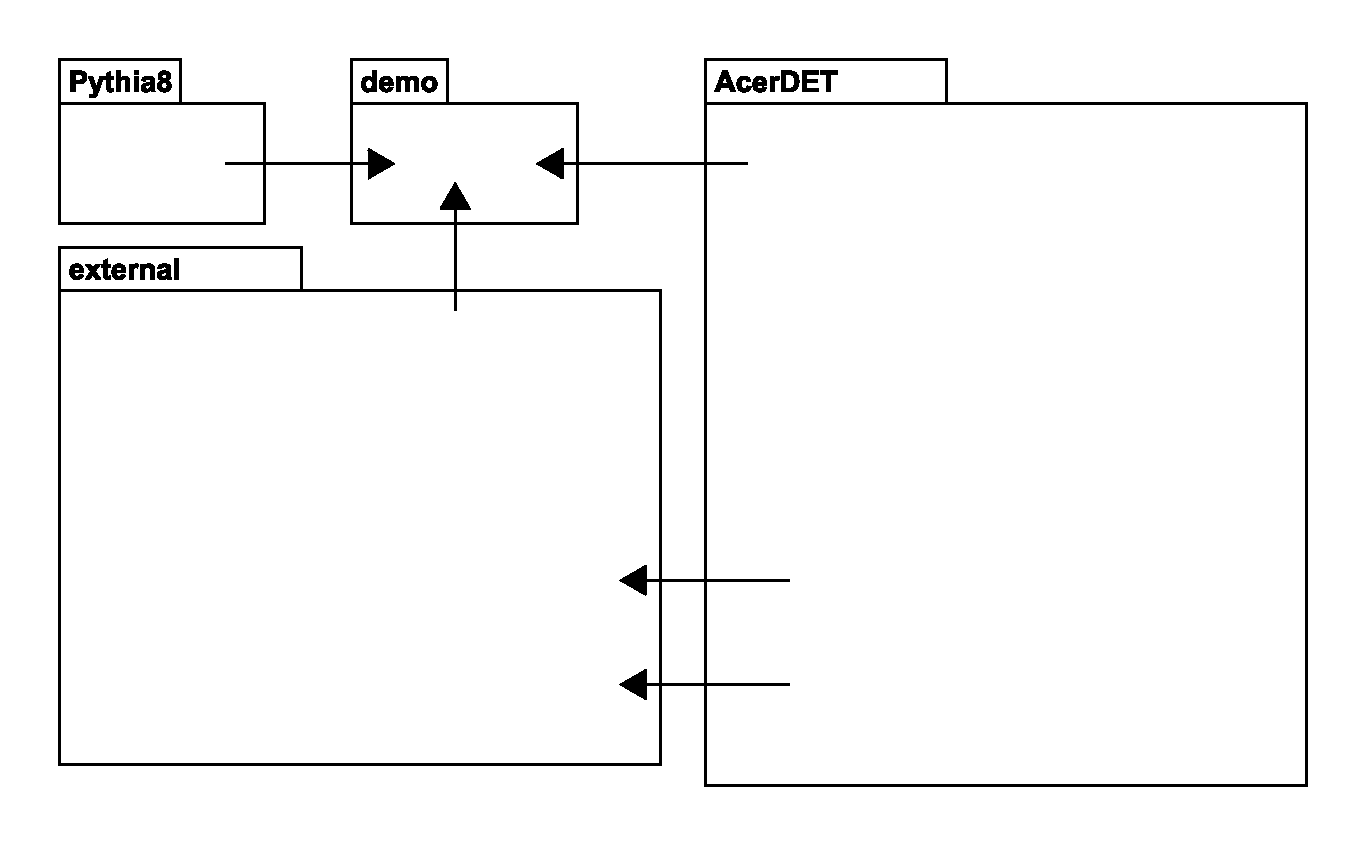
\includegraphics[width=15.0cm,angle=0]{acerdet_structure.eps}\\
}
\end{center}
\caption{\em
Structure of AcerDET package.
\label{acerDETstructure}} 
\end{Fighere}


{\tt AcerDET } is designed to be an universal tool. It does not depend on any external 
library (except {\tt C++ STL}). In order to provide functionalities not built-in directly 
in {\tt AcerDET}, it provides a set of interfaces.

Instantiation of {\tt AcerDET} requires providing instances of such interfaces. Because of 
separation between analyse logic and data structures {\tt AcerDET} might work with a various 
number of external libraries.

The {\tt AcerDET} package provides a set of default implementations for its interfaces, 
grouped in {\tt AcerDET::external} subpackage containing:
\begin{itemize}

\item {\tt Root\_HistogramManager} -- a default implementation of {\tt IHistogramManager} 
interface. Provides methods for storing weighted data in named histograms. 
For more details see {\tt AcerDET::core::IHistogramManager}.

\item {\tt Pythia8\_ParticleDataProviderFactory} -- a default implementation of 
{\tt IParticleDataProviderFactory} interface. Represents a particle types database, 
providing particle charge, name, etc. For more details see {\tt AcerDET::core::ParticleDataProvider}.

\item {\tt HepMC\_InputConverter} -- static class converting {\tt HepMC} event record 
to {\tt AcerDET} internal representation of input record. For more details see 
{\tt AcerDET::io::InputRecord}.

\item {\tt Root\_NTupleManager} -- wrapper for {\tt ROOT}'s NTuple. Provides methods for 
storing and saving weighted events. The {\tt demo} uses it like an external database.

\end{itemize}

The {\tt acerdet.dat} file (configuration file for {\tt AcerDET} package) resides in
subdirectory {\tt acerdet\_dat}. Source code resides in {\tt
acerdet\_src} which has one level deeper internal structure (see README there). 
Interfaces to external libraries are in directory {\tt acerdet\_external}
The library will be created in {\tt acerdet\_src} directory, provided is also
example of the main program {\tt  demo.cpp} to execute {\tt AcerDET} algorithms
with  {\tt PYTHIA 8.1} generator:

\begin{itemize}
\item
Struture of directory {\bf acerdet}
{\scriptsize
\begin{verbatim}  
  -rw-rw-r--  1 erichter erichter    3703 Jun 10 16:07 acerdet.dat
  -rw-rw-r--  1 erichter erichter      65 Jun 10 16:07 common.inc
  drwxrwxr-x  2 erichter erichter    4096 Jun 12 10:31 conf
  -rw-rw-r--  1 erichter erichter    2719 Jun 10 17:25 demo.cpp
  -rw-rw-r--  1 erichter erichter     590 Jun 10 16:07 demoCreateConfig.cpp
  drwxrwxr-x  3 erichter erichter    4096 Jun 12 10:31 external
  -rw-rw-r--  1 erichter erichter     861 Jun 10 16:08 external.inc
  drwxrwxr-x  8 erichter erichter    4096 Jun 12 17:55 .git
  -rw-rw-r--  1 erichter erichter      74 Jun 10 16:09 .gitignore
  -rw-rw-r--  1 erichter erichter     848 Jun 10 16:07 Makefile
  -rw-rw-r--  1 erichter erichter     204 Jun 10 16:08 path.inc
  -rw-rw-r--  1 erichter erichter     274 Jun 10 16:07 README
  -rw-rw-r--  1 erichter erichter      69 Jun 10 16:07 setup.sh
  drwxrwxr-x  6 erichter erichter    4096 Jun 12 10:31 src
\end{verbatim} 
}
\item
Struture of directory {\bf acerdet/src} (after compilation using 'make')
{\scriptsize
\begin{verbatim}  
  -rw-rw-r-- 1 erichter erichter    4078 Jun 10 17:25 AcerDET.cpp
  -rw-rw-r-- 1 erichter erichter    3994 Jun 10 17:25 AcerDET.h
  -rw-rw-r-- 1 erichter erichter  264412 Jun 10 17:25 AcerDET.o
  drwxrwxr-x 2 erichter erichter    4096 Jun 12 10:31 analyse
  drwxrwxr-x 2 erichter erichter    4096 Jun 10 17:25 conf
  drwxrwxr-x 2 erichter erichter    4096 Jun 11 19:14 core
  -rw-rw-r-- 1 erichter erichter   99229 Jun 10 16:08 doxygen.config
  drwxrwxr-x 2 erichter erichter    4096 Jun 10 17:25 io
  -rw-rw-r-- 1 erichter erichter 5538158 Jun 12 10:31 libAcerDET.a
  -rwxrwxr-x 1 erichter erichter 3803523 Jun 12 10:31 libAcerDET.so
  -rw-rw-r-- 1 erichter erichter    1689 Jun 10 16:07 Makefile
  -rw-rw-r-- 1 erichter erichter     132 Jun 10 16:08 path.inc
  -rw-rw-r-- 1 erichter erichter     252 Jun 10 16:07 README
\end{verbatim} 
}
\end{itemize}


To execute the package following actions should be taken:
\begin{itemize}
\item
In subdirectory {\tt acerdet} edit files {\tt  external.inc} and {path.inc}.
Then type: {\it make }. It will
compile the code and create the {\tt src/libAcerDET.a} and {\tt src/libAcerDET.so}.
It will create also demo executable {\tt demo.exe}
\item
To execute, type  {\tt ./demo.exe  conf/XXX.conf nEvent}
where  {\tt conf/XXX.conf} stands for file configuring generated process and 
{\tt nEvent} is a integer number of required events to be generated.
\item
Output will be stored in file  {\tt conf/XXX.conf.root}

\end{itemize}


%%%%%%%%%%%%%%%%%%%%%%%%%%%%%%%%%%%%%%%%%%%%%%%%
\subsection{Development}
%%%%%%%%%%%%%%%%%%%%%%%%%%%%%%%%%%%%%%%%%%%%%%%%

Regarding modifications in {\tt AcerDET} algorithms, package users are able to 
develop own extensions to our main algorithm. As it was shown in previous section 
{\tt AcerDET} provides a set of interfaces to implement in order to use the package.
{\tt AcerDET::external} subpackage contains default implementations of those interfaces, 
but user may develop his own implementations. For instance if someone wants to use 
other histogram manager, it is enough to create new class inheriting from 
{\tt AcerDET::core::IHistogramManager} and pass it's instance when create new {\tt AcerDET} 
instance (as it is shown in {\tt demo.cpp}).

{\scriptsize
\begin{verbatim}  
const std::string configFileName = "acerdet.dat";
Configuration configuration = Configuration::fromFile( configFileName );
IParticleDataProviderFactory *pdpFactory =
	new external::Pythia8_ParticleDataProviderFactory();
IHistogramManager *histoManager =
	new external::Root_HistogramManager(); // HERE USE OWN INSTANCE
external::Root_NTupleManager nTuple;

AcerDET acerDet(
	configuration,
	pdpFactory,
	histoManager 
);
\end{verbatim} 
}

Analoguously user may use own instance of {\tt IParticleDataProviderFactory}.
{\tt ROOT} NTuple is used in demo like na external database, so using other 
databases is possible in similiar way.
Distributed demo version uses {\tt HepMC} as input data standard, while 
{\tt AcerDET} uses its own input format. Default conversion algoritm is 
placed in {\tt AcerDET::external::HepMC\_InputConverter}. In order to use 
other input format, similiar converter to {\tt AcerDET} input format is required.


\newpage
%%%%%%%%%%%%%%%%%%%%%%%%%%%%%%%%%%%%%%%%%%%%%%%%
\section{List of input parameters: {\tt acerdet.dat} file}
%%%%%%%%%%%%%%%%%%%%%%%%%%%%%%%%%%%%%%%%%%%%%%%%
{\scriptsize
\begin{verbatim}  
Flag.HistogramID                10000        ....id for histograms
Flag.Smearing                   1            ....smearing on=1, off=0
Flag.B-Field                    1            ....B-field  on=1, off=0
Flag.SUSY_LSP_Particle          66           ....code for SUSY LSP particle
Flag.BC-JetsLabeling            1            ....b- and c-jets labeling on=1, off=0
Flag.Tau-JetsLabeling           1            ....tau-jets labeling on=1, off=0
Flag.JetCalibration             1            ....jet calibration  on=1, off=0

Cell.RapidityCoverage           5.000        ....rapidity coverage
Cell.MinpT                      0.500        ....min p_T for B-field
Cell.MinEt                      0.000        ....min E_T for cell 
Cell.EtaTransition              3.200        ....eta transition in cells granularity
Cell.GranularityEta             0.100        ....granularity in eta (within Cell.EtaTransition), 2x outside
Cell.GranularityPhi             0.100        ....granularity in phi (within Cell.EtaTransition), 2x outside

Cluster.MinEt                   5.000        ....minimum E_T for cluster
Cluster.ConeR                   0.400        ....cone R for clustering 
Cluster.RapidityCoverage        5.000        ....rapidity coverage
Cluster.MinEtInit               1.500        ....min E_T for cluster initiator

Muon.MinMomenta                 6.000        ....minimum muon-momenta to be detected
Muon.MaxEta                     2.500        ....maximum muon eta to be detected
Muon.MinIsolRlj                 0.400        ....min R_lj for muon-isolation
Muon.ConeR                      0.200        ....R_cone for energy deposition 
Muon.MaxEnergy                  10.000       ....max energy deposition for isol

Photon.MinMomenta               5.000        ....minimum photon-momenta to be isol
Photon.MaxEta                   2.500        ....maximum photon eta to be isol
Photon.MinJetsRlj               0.150        ....min R_lj for photon-jet
Photon.MinIsolRlj               0.400        ....min R_lj for photon-isolation
Photon.ConeR                    0.200        ....R_cone for energy deposition 
Photon.MaxEnergy                10.000       ....max energy deposition for isol

Electron.MinMomenta             5.000        ....minimum electron-momenta to be isol
Electron.MaxEta                 2.500        ....maximum electron eta to be isol
Electron.MinJetsRlj             0.150        ....min R_lj for electron-jet
Electron.MinIsolRlj             0.400        ....min R_lj for electron-isolation
Electron.ConeR                  0.200        ....R_cone for energy deposition 
Electron.MaxEnergy              10.000       ....max energy deposition for isol

Jets.MinEnergy                  10.000       ....jets energy_min  threshold
Jets.RapidityCoverage           5.000        ....rapidity coverage for jets

BJets.MinMomenta                5.000        ....minimum b-quark pT (after FSR) momenta for b-jet label
BJets.MaxEta                    2.500        ....maximum b-quark eta for  b-jet label
BJets.MaxRbj                    0.200        ....max R_bj for b-jet label

CJets.MinMomenta                5.000        ....minimum c-quark pT (after FSR) momenta for c-jet label
CJets.MaxEta                    2.500        ....maximum c-quark eta for  c-jet label
CJets.MaxRcj                    0.200        ....max R_cj for c-jet label

Tau.MinpT                       10.000       ....minimum tau-had pT for  tau-jet label
Tau.MaxEta                      2.500        ....maximum tau-eta for  tau-jet label
Tau.MinR                        0.300        ....max R_tauj for tau-jet
Tau.MaxR                        0.900        ....max R_tauj for tau-jet

Misc.MinEt                      0.000        ....min E_T for energy in cell to count unused cell
\end{verbatim}  
}

\newpage
%%%%%%%%%%%%%%%%%%%%%%%%%%%%%%%%%%%%%%%%%%%%%%%%
\section{Reconstructed entities}
%%%%%%%%%%%%%%%%%%%%%%%%%%%%%%%%%%%%%%%%%%%%%%%%

Reconstructed entities are stored as vectors of {\tt ObjectData} (for isolated photon, muons, electrons),
as {\tt CellData} (for cells), as {\tt JetData} (for jets) and {\tt MisData} for missing energy. 
Objects in each category of  {\tt ObjectData} and  {\tt JetData} are ordered 
with the decreasing transverse momenta.

\subsection{ ObjectData }

For  {\tt ObjectData} stored is information of the {\tt pdg\_id}, 
so the information of the charge is preserved, {\tt eta}, {\tt phi} and {\tt pT}
which allows to recalculate full kinematics assuming that mass is equal to zero, 
and the internal flag  {\tt alreadyUsed} needed for calculating missing tranverse 
energy for the event. 

\subsection{ JetData }

For {\tt JetData} stored is information on the {\tt type} which flags if a given
jet is b-quark tagged, c-quark tagged or matched with hadronic-tau decays.
The angular kinematic variables {\tt eta}, {\tt phi} and {\tt eta\_rec}, {\tt phi\_rec}
and {\tt pT}.  

\subsection{ MisData }

For {\tt MisData } stored is information on reconstructed momenta both transverse
components of electrons, muons, photons, clusters and jets, {\tt PXSUM, PYSUM}, on reconstructed
total tranverse components i.e.
after adding non-clusterd cells  {\tt PXREC, PYREC}, sum of transverse momenta components, 
the reconstructed transverse momenta {\tt SUMET}, the transverse components of momenta 
of neutrinos and invisible particles (as defined by the user) in the event {\tt PXNUES, PYNUES}
and finally sum of the total transverse energy components deposited in the
calorimeter {\tt PXXCALO, PYYCALO}.

%%%%%%%%%%%%%%%%%%%%%%%%%%%%%%%%%%%%%%%%%%%%%%%%
\section{Content of the {\tt ACDTree} }
%%%%%%%%%%%%%%%%%%%%%%%%%%%%%%%%%%%%%%%%%%%%%%%%

Reconstructed objects and, for convenience of the analysis, also partial information on 
generated event are stored in the format of {\tt ROOT} tree, the {\tt ACDTree}.

\begin{itemize}
\item
Generator info: Event weight and identifier for generated process.
\item
Generated particles: stored are those participating in the {\it hard-scattering},
which is defined using {\tt isHardProcess} method and  flags: {\tt PS\_Beam}, {\tt PS\_HISTORY}.
Stored are 4-momenta, and {\tt pdg\_id} code. 
\item
Isolated photons, electrons, muons: stored are 4-momenta, and {\tt pdg\_id} code. 
\item
Jets:  stored are 4-momenta, the {\tt pdg\_id} code indicate if jet was labeled as -batteg, c-tagged 
or hadronic-decay of tau lepton.
\item
Missing energy: stored are transverse momenta components of missing energy, invisible energy
and energy reconstructed in the calorimeter.
\end{itemize}

Additional information, if required, can be also extracted from
the  internal variables of simulation and reconstruction
algorithms: eg. on used/unused cells, non-isolated muons, 
unused clusters, etc. and added to the {\tt ACDTree}.

%%%%%%%%%%%%%%%%%%%%%%%%%%%%%%%%%%%%%%%%%%%%%%%%
\section{Parametrisation for energy/momenta resolution}
%%%%%%%%%%%%%%%%%%%%%%%%%%%%%%%%%%%%%%%%%%%%%%%%

\subsection{Function RESPHO}

The parametrisation for photon energy resolution assumes only 
energy dependence and the Gaussian
smearing with $10\%/\sqrt{E_{\gamma}}$ resolution.
\begin{equation}
 E_{\gamma}^{smeared}  = 
E_{\gamma}^{true} \cdot (1+ r_n \cdot \frac{0.10}{\sqrt{E_{\gamma}^{true}}}). 
\end{equation}
Where $r_n$ is the random number generated according to the Gaussian
distribution (normal distribution from Standard C++ library).
All 4-momenta components of the photon are smeared with the same
resolution so the direction of the photon is not altered. 

\subsection{Function RESELE}

The parametrisation for electron energy resolution assumes only 
energy dependence and the Gaussian
smearing with $12\%/\sqrt{E_{e}}$ resolution.
\begin{equation}
 E_{e}^{smeared}  = 
E_{e}^{true} \cdot (1+ r_n \cdot \frac{0.12}{\sqrt{E_{e}^{true}}}). 
\end{equation}
Where $r_n$ is the random number generated according to the Gaussian
distribution (normal distribution from Standard C++ library).
All 4-momenta components of the electron are smeared with the same
resolution so the direction of the electron is not altered. 

\subsection{Function RESHAD}

The parametrisation for clusters momenta resolution assumes only 
energy dependence and Gaussian
smearing with $50\%/\sqrt{E_{clu}}$ or $100\%/\sqrt{E_{clu}}$
resolution.
The transition region, $|\eta^{clu}| = CALOTH$  is the same as the 
transition of the cells granularity. \\
For  $|\eta^{clu}| < CALOTH$:
\begin{equation}
 E_{clu}^{smeared}  = 
E_{clu}^{true} \cdot (1+ r_n \cdot \frac{0.50}{\sqrt{E_{clu}^{true}}}). 
\end{equation}
For  $|\eta^{clu}| > CALOTH$:
\begin{equation}
 E_{clu}^{smeared}  = 
E_{clu}^{true} \cdot (1+ r_n \cdot \frac{1.00}{\sqrt{E_{clu}^{true}}}). 
\end{equation}
Where $r_n$ is the random number generated according to the Gaussian
distribution (normal distribution from Standard C++ library).
All 4-momenta components of the muon are smeared with the same
resolution so the direction of the muon is not altered. 

\subsection{Function RESMUO}

The parametrisation for muon momenta resolution assumes only 
transverse momenta dependence and Gaussian
smearing with $0.0005 \cdot pT_{\mu}$ resolution.
\begin{equation}
 pT_{\mu}^{smeared}  = 
pT_{\mu}^{true}/(1+ r_n \cdot 0.0005 \cdot pT_{\mu}^{true}). 
\end{equation}
Where $r_n$ is the random number generated according to the Gaussian
distribution (normal distribution from Standard C++ library).
All 4-momenta components of the muon are smeared with the same
resolution so the direction of the muon is not altered. 

\subsection{Function FLDPHI}

The effect of the magnetic field is included by simple shifting the
$\phi$ position of the charged particles respectively to its
transverse momenta, parametrised as following:
\begin{equation}
 \delta \phi   =  0.5 / pT^{part}. 
\end{equation}
The $ \delta \phi$ is calculated in radians and $pT^{part}$ is
given in $GeV$.
The sign of the  $ \delta \phi$ is the same as the sign of the
particle charge.
Charged particles with  $pT^{part} < 0.5$ GeV are assumed to be
looping in the detector and not depositing energy in the calorimeter.


%%%%%%%%%%%%%%%%%%%%%%%%%%%%%%%%%%%%%%%%%%%%%%%%
\section{Some formulas}
%%%%%%%%%%%%%%%%%%%%%%%%%%%%%%%%%%%%%%%%%%%%%%%%

We work with the assumptions of massless reconstructed objets. The
following relations were used to translate between $(p_T, \eta, \phi)$
coordinates and four-momenta $(p_x, p_y, p_z, E)$.

\begin{equation}
 p_x=p_T \cdot cos(\phi) 
\end{equation}
\begin{equation}
 p_y=p_T \cdot sin(\phi)
\end{equation}
\begin{equation}
 p_z=p_T \cdot cosh(\eta) 
\end{equation}
\begin{equation}
 E  =p_T \cdot sinh(\eta)
\end{equation}

\begin{equation}
 p_T = \sqrt{p_x^2 + p_y^2}
\end{equation}
\begin{equation}
\eta = sign(\ln{\frac{\sqrt{p_T^2+p_z^2}+|p_z|}{p_T}},p_z)
\end{equation}
\begin{equation}
 \phi = asinh(p_y/\sqrt{p_x^2+p_y^2}) 
\end{equation}

\newpage
%%%%%%%%%%%%%%%%%%%%%%%%%%%%%%%%%%%%%%%%%%%%%%%%
\section{Output content}
%%%%%%%%%%%%%%%%%%%%%%%%%%%%%%%%%%%%%%%%%%%%%%%%

%%%%%%%%%%%%%%%%%%%%%%%%%%%%%%%%%%%%%%%%%%%%%%%%
\subsection{Output ACDTree content: {\tt acerdet.ntup} file}
%%%%%%%%%%%%%%%%%%%%%%%%%%%%%%%%%%%%%%%%%%%%%%%%
The content of the ntuple is exactly as described in the previous
section. As an auxiliary info, within the stored information,
could be provided code on the generated process, {\tt IDPROC}.

{\scriptsize
\begin{verbatim}  
******************************************************************************
*Tree    :ACDTree   : ACDTree                                                *
*Entries :       10 : Total =           30521 bytes  File  Size =      13140 *
*        :          : Tree compression factor =   1.00                       *
******************************************************************************
*Br    0 :ProcessID : ProcessID/I                                            *
*Entries :       10 : Total  Size=        609 bytes  File Size  =        119 *
*Baskets :        1 : Basket Size=      32000 bytes  Compression=   1.00     *
*............................................................................*
*Br    1 :part_n    : part_n/I                                               *
*Entries :       10 : Total  Size=        594 bytes  File Size  =        116 *
*Baskets :        1 : Basket Size=      32000 bytes  Compression=   1.00     *
*............................................................................*
*Br    2 :part_pdgId : vector<int>                                           *
*Entries :       10 : Total  Size=       1358 bytes  File Size  =        860 *
*Baskets :        1 : Basket Size=      32000 bytes  Compression=   1.00     *
*............................................................................*
*Br    3 :part_px   : vector<float>                                          *
*Entries :       10 : Total  Size=       1343 bytes  File Size  =        857 *
*Baskets :        1 : Basket Size=      32000 bytes  Compression=   1.00     *
*............................................................................*
*Br    4 :part_py   : vector<float>                                          *
*Entries :       10 : Total  Size=       1343 bytes  File Size  =        857 *
*Baskets :        1 : Basket Size=      32000 bytes  Compression=   1.00     *
*............................................................................*
*Br    5 :part_pz   : vector<float>                                          *
*Entries :       10 : Total  Size=       1343 bytes  File Size  =        857 *
*Baskets :        1 : Basket Size=      32000 bytes  Compression=   1.00     *
*............................................................................*
*Br    6 :part_E    : vector<float>                                          *
*Entries :       10 : Total  Size=       1338 bytes  File Size  =        856 *
*Baskets :        1 : Basket Size=      32000 bytes  Compression=   1.00     *
*............................................................................*
*Br    7 :ele_n     : ele_n/I                                                *
*Entries :       10 : Total  Size=        589 bytes  File Size  =        115 *
*Baskets :        1 : Basket Size=      32000 bytes  Compression=   1.00     *
*............................................................................*
*Br    8 :ele_pdgId : vector<int>                                            *
*Entries :       10 : Total  Size=        721 bytes  File Size  =        227 *
*Baskets :        1 : Basket Size=      32000 bytes  Compression=   1.00     *
*............................................................................*
*Br    9 :ele_px    : vector<float>                                          *
*Entries :       10 : Total  Size=        706 bytes  File Size  =        224 *
*Baskets :        1 : Basket Size=      32000 bytes  Compression=   1.00     *
*............................................................................*
*Br   10 :ele_py    : vector<float>                                          *
*Entries :       10 : Total  Size=        706 bytes  File Size  =        224 *
*Baskets :        1 : Basket Size=      32000 bytes  Compression=   1.00     *
*............................................................................*
*Br   11 :ele_pz    : vector<float>                                          *
*Entries :       10 : Total  Size=        706 bytes  File Size  =        224 *
*Baskets :        1 : Basket Size=      32000 bytes  Compression=   1.00     *
*............................................................................*
*Br   12 :ele_E     : vector<float>                                          *
*Entries :       10 : Total  Size=        701 bytes  File Size  =        223 *
*Baskets :        1 : Basket Size=      32000 bytes  Compression=   1.00     *
*............................................................................*
*Br   13 :muo_n     : muo_n/I                                                *
*Entries :       10 : Total  Size=        589 bytes  File Size  =        115 *
*Baskets :        1 : Basket Size=      32000 bytes  Compression=   1.00     *
*............................................................................*
*Br   14 :muo_pdgId : vector<int>                                            *
*Entries :       10 : Total  Size=        721 bytes  File Size  =        227 *
*Baskets :        1 : Basket Size=      32000 bytes  Compression=   1.00     *
*............................................................................*
*Br   15 :muo_px    : vector<float>                                          *
*Entries :       10 : Total  Size=        706 bytes  File Size  =        224 *
*Baskets :        1 : Basket Size=      32000 bytes  Compression=   1.00     *
*............................................................................*
*Br   16 :muo_py    : vector<float>                                          *
*Entries :       10 : Total  Size=        706 bytes  File Size  =        224 *
*Baskets :        1 : Basket Size=      32000 bytes  Compression=   1.00     *
*............................................................................*
*Br   17 :muo_pz    : vector<float>                                          *
*Entries :       10 : Total  Size=        706 bytes  File Size  =        224 *
*Baskets :        1 : Basket Size=      32000 bytes  Compression=   1.00     *
*............................................................................*
*Br   18 :muo_E     : vector<float>                                          *
*Entries :       10 : Total  Size=        701 bytes  File Size  =        223 *
*Baskets :        1 : Basket Size=      32000 bytes  Compression=   1.00     *
*............................................................................*
*Br   19 :pho_n     : pho_n/I                                                *
*Entries :       10 : Total  Size=        589 bytes  File Size  =        115 *
*Baskets :        1 : Basket Size=      32000 bytes  Compression=   1.00     *
*............................................................................*
*Br   20 :pho_pdgId : vector<int>                                            *
*Entries :       10 : Total  Size=        721 bytes  File Size  =        227 *
*Baskets :        1 : Basket Size=      32000 bytes  Compression=   1.00     *
*............................................................................*
*Br   21 :pho_px    : vector<float>                                          *
*Entries :       10 : Total  Size=        706 bytes  File Size  =        224 *
*Baskets :        1 : Basket Size=      32000 bytes  Compression=   1.00     *
*............................................................................*
*Br   22 :pho_py    : vector<float>                                          *
*Entries :       10 : Total  Size=        706 bytes  File Size  =        224 *
*Baskets :        1 : Basket Size=      32000 bytes  Compression=   1.00     *
*............................................................................*
*Br   23 :pho_pz    : vector<float>                                          *
*Entries :       10 : Total  Size=        706 bytes  File Size  =        224 *
*Baskets :        1 : Basket Size=      32000 bytes  Compression=   1.00     *
*............................................................................*
*Br   24 :pho_E     : vector<float>                                          *
*Entries :       10 : Total  Size=        701 bytes  File Size  =        223 *
*Baskets :        1 : Basket Size=      32000 bytes  Compression=   1.00     *
*............................................................................*
*Br   25 :jet_n     : jet_n/I                                                *
*Entries :       10 : Total  Size=        589 bytes  File Size  =        115 *
*Baskets :        1 : Basket Size=      32000 bytes  Compression=   1.00     *
*............................................................................*
*Br   26 :jet_pdgId : vector<int>                                            *
*Entries :       10 : Total  Size=        877 bytes  File Size  =        383 *
*Baskets :        1 : Basket Size=      32000 bytes  Compression=   1.00     *
*............................................................................*
*Br   27 :jet_px    : vector<float>                                          *
*Entries :       10 : Total  Size=        862 bytes  File Size  =        380 *
*Baskets :        1 : Basket Size=      32000 bytes  Compression=   1.00     *
*............................................................................*
*Br   28 :jet_py    : vector<float>                                          *
*Entries :       10 : Total  Size=        862 bytes  File Size  =        380 *
*Baskets :        1 : Basket Size=      32000 bytes  Compression=   1.00     *
*............................................................................*
*Br   29 :jet_pz    : vector<float>                                          *
*Entries :       10 : Total  Size=        862 bytes  File Size  =        380 *
*Baskets :        1 : Basket Size=      32000 bytes  Compression=   1.00     *
*............................................................................*
*Br   30 :jet_E     : vector<float>                                          *
*Entries :       10 : Total  Size=        857 bytes  File Size  =        379 *
*Baskets :        1 : Basket Size=      32000 bytes  Compression=   1.00     *
*............................................................................*
*Br   31 :pxmiss    : pxmiss/F                                               *
*Entries :       10 : Total  Size=        594 bytes  File Size  =        116 *
*Baskets :        1 : Basket Size=      32000 bytes  Compression=   1.00     *
*............................................................................*
*Br   32 :pymiss    : pymiss/F                                               *
*Entries :       10 : Total  Size=        594 bytes  File Size  =        116 *
*Baskets :        1 : Basket Size=      32000 bytes  Compression=   1.00     *
*............................................................................*
*Br   33 :pxnue     : pxnue/F                                                *
*Entries :       10 : Total  Size=        589 bytes  File Size  =        115 *
*Baskets :        1 : Basket Size=      32000 bytes  Compression=   1.00     *
*............................................................................*
*Br   34 :pynue     : pynue/F                                                *
*Entries :       10 : Total  Size=        589 bytes  File Size  =        115 *
*Baskets :        1 : Basket Size=      32000 bytes  Compression=   1.00     *
*............................................................................*
*Br   35 :pxcalo    : pxcalo/F                                               *
*Entries :       10 : Total  Size=        594 bytes  File Size  =        116 *
*Baskets :        1 : Basket Size=      32000 bytes  Compression=   1.00     *
*............................................................................*
*Br   36 :pycalo    : pycalo/F                                               *
*Entries :       10 : Total  Size=        594 bytes  File Size  =        116 *
*Baskets :        1 : Basket Size=      32000 bytes  Compression=   1.00     *
*............................................................................*
\end{verbatim}
} 

\newpage
%%%%%%%%%%%%%%%%%%%%%%%%%%%%%%%%%%%%%%%%%%%%%%%%
\subsection{Control printout}
%%%%%%%%%%%%%%%%%%%%%%%%%%%%%%%%%%%%%%%%%%%%%%%%

{\scriptsize
\begin{verbatim}  
**********************************************************
*                  AcerDET, version: 2.0                 *
*                 Released at: 30.06.2015                *
*                                                        *
*  Simplied event simulation and reconstruction package  *
*                                                        *
*           by E. Richter-Was (Institute of Physics)     *
*          and P. Mikos (Theoretical Computer Science)   *
*         Jagiellonian University, Cracow, Poland        *
**********************************************************

 Initial configuration:
*************************************
*                                   *
*     *************************     *
*     ***   analyse::Cell   ***     *
*     *************************     *
*                                   *
*************************************

	 clusters definition ...
 eta coverage  5.000000
 E_T_min cell thresh 0.000000
 eta gran. transition 3.200000
 gran in eta(central) 0.100000
 gran in phi(central) 0.100000

	 B field apply ....
 B-field on
 p_T min non looping 0.500000

****************************************
*                                      *
*     ****************************     *
*     ***   analyse::Cluster   ***     *
*     ****************************     *
*                                      *
****************************************

	 clusters definition ...
 E_T_min cluster 5.000000
 E_T_min cell initia 1.500000
 R cone 0.400000
 eta coverage 5.000000
 eta gran. transition 3.200000

*************************************
*                                   *
*     *************************     *
*     ***   analyse::Muon   ***     *
*     *************************     *
*                                   *
*************************************

	... muon isolation ...
min. muon p_T 6.000000
max. muon eta 2.500000
min R_lj for isolation 0.400000
R for energy deposit 0.200000
max E_dep for isolation 10.000000
smearing on
\end{verbatim}  
\newpage
\begin{verbatim}

*****************************************
*                                       *
*     *****************************     *
*     ***   analyse::Electron   ***     *
*     *****************************     *
*                                       *
*****************************************

	... electron isolation ...
min. lepton p_T 5.000000
max. lepton eta 2.500000
max R_ej for ele-clu 0.150000
min R_lj for isolation 0.400000
R for energy deposit 0.200000
max E_dep for isolation 10.000000
smearing on

***************************************
*                                     *
*     ***************************     *
*     ***   analyse::Photon   ***     *
*     ***************************     *
*                                     *
***************************************

	... photon isolation ...
min. photon p_T 5.000000
max. photon eta 2.500000
max R_gam-clust 0.150000
min R_isol 0.400000
R for energy deposit 0.200000
max E_dep for isolation 10.000000
smearing on

************************************
*                                  *
*     ************************     *
*     ***   analyse::Jet   ***     *
*     ************************     *
*                                  *
************************************

	 clusters definition ....
 R cone 0.400000
	 jets definition ....
 E_T_jets [GeV] 10.000000
 eta coverage jets 5.000000
 smearing on
 B-field on

\end{verbatim}
\newpage
\begin{verbatim}

************************************
*                                  *
*     ************************     *
*     ***   analyse::Mis   ***     *
*     ************************     *
*                                  *
************************************

	 muon coverage
 min. muon p_T 6.000000
 max. muon eta 2.500000
	 unused cells ...
 smearing on
 cells threshold 10.000000
	 invisible particles ...
 KF code for invis 66

*************************************
*                                   *
*     *************************     *
*     ***   analyse::BJet   ***     *
*     *************************     *
*                                   *
*************************************

	... jets labeling ...
labeling on/off on
	bjets ...
min b-quark p_T 5.000000
max b-quark eta 2.500000
max R_bj for b-jets 0.200000

*************************************
*                                   *
*     *************************     *
*     ***   analyse::CJet   ***     *
*     *************************     *
*                                   *
*************************************

	... jets labeling ...
labeling on/off on
	cjets ...
min c-quark p_T 5.000000
max c-quark eta 2.500000
max R_cj for c-jets 0.200000

************************************
*                                  *
*     ************************     *
*     ***   analyse::Tau   ***     *
*     ************************     *
*                                  *
************************************

	... tau-jets labeling ...
labeling on/off on
	tau-jets ...
min tau-had p_T 10.000000
max tau-had eta 2.500000
max R_tauj for tau-jets 0.300000
tau-had frac. of jet 0.900000

\end{verbatim}
\newpage
\begin{verbatim}

********************************************
*                                          *
*     ********************************     *
*     ***   analyse::Calibration   ***     *
*     ********************************     *

	 jets calibration ....
 calibration on
\end{verbatim}  
}

%%%%%%%%%%%%%%%%%%%%%%%%%%%%%%%%%%%%%%%%%%%%%%%%%%
\subsection{Control histograms: XXX.conf.root  file}
%%%%%%%%%%%%%%%%%%%%%%%%%%%%%%%%%%%%%%%%%%%%%%%%%%

Below is the list of control histograms which monitors performance of
the simulation/reconstruction. The are store together with {\tt ACDTree}
tuple in file XXX.conf.root.
\scriptsize{
\begin{verbatim}  
  KEY: TH1F	hist10000;1	Cell: multiplicity
  KEY: TH1F	hist10101;1	Cluster: multiplicity
  KEY: TH1F	hist10111;1	Cluster: delta eta cluster barycentre
  KEY: TH1F	hist10112;1	Cluster: delta phi cluster barycentre
  KEY: TH1F	hist10113;1	Cluster: delta r   cluster barycentre
  KEY: TH1F	hist10123;1	Cluster: delta r   cluster HPparton
  KEY: TH1F	hist10114;1	Cluster: pTclu/SumpT particle
  KEY: TH1F	hist10124;1	Cluster: pTclu/SumpT HP parton
  KEY: TH1F	hist10210;1	Muon: muon multiplicity NOISOLATED
  KEY: TH1F	hist10211;1	Muon: muon multiplicity ISOLATED
  KEY: TH1F	hist10221;1	Muon: muon multiplicity HP
  KEY: TH1F	hist10231;1	Muon: muon multiplicity HP+ISOL
  KEY: TH1F	hist10311;1	Electron: multiplicity ISOLATED
  KEY: TH1F	hist10321;1	Electron: multiplicity HP
  KEY: TH1F	hist10331;1	Electron: multiplicity HP+ISOL
  KEY: TH1F	hist10411;1	Photon: photon multiplicity ISOLATED
  KEY: TH1F	hist10421;1	Photon: photon multiplicity HP
  KEY: TH1F	hist10431;1	Photon: photon multiplicity HP+ISOL
  KEY: TH1F	hist10501;1	Jet: multiplicity
  KEY: TH1F	hist10511;1	Jet: delta phi jet-barycentre
  KEY: TH1F	hist10512;1	Jet: delta eta jet-barycentre
  KEY: TH1F	hist10513;1	Jet: delta r jet-barycentre
  KEY: TH1F	hist10514;1	Jet: delta r jet- HP parton
  KEY: TH1F	hist10523;1	Jet: pTjet/pT particles in Rcone
  KEY: TH1F	hist10524;1	Jet: pTjet/pT HP parton
  KEY: TH1F	hist10611;1	Mis: reconstructed p_T 
  KEY: TH1F	hist10612;1	Mis: reconstructed p_T + cells
  KEY: TH1F	hist10613;1	Mis: reconstructed pTmiss
  KEY: TH1F	hist10621;1	Mis: true p_T invisible
  KEY: TH1F	hist10711;1	BJet: b-jets multiplicity
  KEY: TH1F	hist10721;1	BJet: b-quarks HP multiplicity
  KEY: TH1F	hist10723;1	BJet: delta r bjet-bquark HP
  KEY: TH1F	hist10724;1	BJet: pTbjet/pTbquark HP
  KEY: TH1F	hist10811;1	CJet: c-jets multiplicity
  KEY: TH1F	hist10821;1	CJet: c-quarks HP multiplicity
  KEY: TH1F	hist10823;1	CJet: delta r cjet-cquark HP
  KEY: TH1F	hist10824;1	CJet: pTcjet/pTcquark HP
  KEY: TH1F	hist10911;1	Tau: tau-jets multiplicity
  KEY: TH1F	hist10921;1	Tau: tau-had multiplicity 
  KEY: TH1F	hist10923;1	Tau: delta r tau-jet, tau-had 
  KEY: TH1F	hist10924;1	Tau: pTtaujet/pTtau-had 
  KEY: TTree	ACDTree;1	ACDTree                 
\end{verbatim}  
}

\end{document}

















